\documentclass{report}
\usepackage[utf8]{inputenc}
\usepackage[colorinlistoftodos,prependcaption]{todonotes}
\usepackage{hyperref}
\usepackage{listings}
\usepackage{xcolor}
\usepackage{graphicx}
\usepackage{float}
\usepackage[nottoc]{tocbibind}

\colorlet{punct}{red!60!black}
\definecolor{background}{HTML}{EEEEEE}
\definecolor{delim}{RGB}{20,105,176}
\colorlet{numb}{magenta!60!black}
\usepackage{pdfpages}


\usepackage{xcolor}
\usepackage{listings}
\setlength\textwidth{140mm}

\lstdefinestyle{DOS}
{
    backgroundcolor=\color{gray},
    basicstyle=\color{white}\ttfamily,
    breaklines=true,
    postbreak=\mbox{\textcolor{red}{$\hookrightarrow$}\space}
}

\lstdefinelanguage{json}{
    basicstyle=\normalfont\ttfamily,
    numbers=left,
    numberstyle=\scriptsize,
    stepnumber=1,
    numbersep=8pt,
    showstringspaces=false,
    breaklines=true,
    frame=lines,
    backgroundcolor=\color{background}
}

% Thesis title in English (exactly as in the formal assignment)
\def\ThesisTitle{Scent of Current Network Overview}
\def\Abbreviation{SOCNETO}

% Author of the thesis
\def\ThesisAuthor{Bc.~Július Flimmel, Bc.~Jaroslav Knotek, Bc.~Lukáš Kolek, Bc.~Petra Vysušilová}

% Year when the thesis is submitted
\def\YearSubmitted{2020}

% Name of the department or institute, where the work was officially assigned
% (according to the Organizational Structure of MFF UK in English,
% or a full name of a department outside MFF)
\def\Department{Department of Software Engineering}

% Is it a department (katedra), or an institute (ústav)?
\def\DeptType{Institute}

% Thesis supervisor: name, surname and titles
\def\Supervisor{doc. RNDr. Irena Holubová, Ph.D.}

% Supervisor's department (again according to Organizational structure of MFF)
\def\SupervisorsDepartment{Department of Software Engineering}



\def\Dedication{%
We would first like to thank to our advisor, Doc. RNDr. Irena Holubová, Ph.D. She devoted a lot of time to to our project and provided us valuable advices and support. We would also like to thank to RNDr. Jakub Yaghob, Ph.D. for his willing help with school clusters. We are grateful Datamole provided its space for our meetings and coding sessions, which helped us to move a lot. Last but not least our thanks belong to Bc. Jiří Suchomel, who suggested real use cases for Socneto and also connected us with other people, which can use Socneto for their use cases.
}

\def\Abstract{%
The aim of the project is to develop a framework for analysis of social
network data. It provides users with functionality to analyse sentiment of
large amounts of data and visualize the results. Data are acquired via
social networks public APIs or custom modules.
}

\def\Keywords{%
{key} {words}
}
\title{Development documentation}
\author{SOCNETO}
\date{February 2020}

\begin{document}
%%% Title page of the thesis and other mandatory pages

%%% Title page of the thesis

\pagestyle{empty}
%\hypersetup{pageanchor=false}
\begin{center}



\vspace{-8mm}
\vfill

{\bf\Large SOFTWARE PROJECT}

\vfill

\vfill
{\LARGE\ThesisAuthor}

\vspace{15mm}

{\LARGE\bfseries\ThesisTitle}

\vfill
\centerline{\mbox{
\includegraphics[width=40mm]{diagrams/fsocneto_icon.png}}}
\vfill
Prague \YearSubmitted
\end{center}
\newpage




%%% Mandatory information page of the thesis

%\openright

\vbox to 0.5\vsize{
\setlength\parindent{0mm}
\setlength\parskip{5mm}

Project name:
\ThesisTitle

Authors:
\ThesisAuthor

Supervisor:
\Supervisor, \SupervisorsDepartment

Abstract:
\Abstract

\vss}

\newpage
%%% Dedication

%\openright

\noindent
\Dedication

%\openright
\pagestyle{plain}
\pagenumbering{arabic}
\setcounter{page}{1}

%\maketitle
\tableofcontents

\chapter{Introduction}

The document covers the development phase of the software project. Documentation starts with a comparison of Socneto and other social network analysis tools, then there are described real-world use cases, followed by architecture and its components, topic modeling and sentiment analysis development description, platform extensibility and the final discussion.

\section{Team}

Bc. Jaroslav Knotek
\begin{itemize}
\renewcommand\labelitemi{--}
    \item Subject of study: Software and Data Engineering
    \item Socneto components: Acquirers, Job Management service, Analysers, Architecture and Use Cases
\end{itemize}
Bc. Julius Flimmel
\begin{itemize}
\renewcommand\labelitemi{--}
    \item Subject of study: Computer Graphics and Game Development
    \item Socneto components: Frontend, Backend and Deployment
\end{itemize}
Bc. Petra Vysušilová
\begin{itemize}
\renewcommand\labelitemi{--}
    \item Subject of study: Artificial Intelligence
    \item Socneto components: Sentiment analysis, Topic modeling, LaTeX master
\end{itemize}
Bc. Lukáš Kolek
\begin{itemize}
\renewcommand\labelitemi{--}
    \item Subject of study: Software and Data Engineering
    \item Socneto components: Storage, Monitoring and Architecture
\end{itemize}


\chapter{Project Overview}

Socneto is a framework for analysing data from social networks for a given topic. Socneto can be extended with custom data acquirers and custom analyser. Socneto supports two major social networks: Twitter\footnote{\url{www.twitter.com}} and Reddit\footnote{\url{www.reddit.com}}; and two data analysers of key topics and sentiment supported in the current version of Socneto. 

% \todo{Možná bych (i jidne v textu) zdůraznila, že ty dvě SN a analyzátory jsou podporované v aktuální verzi SW, ale je možné přidávat další. Obecně tu rozšiřitelnost je potřeba vhodně zdůraznit.} 

\section{Introduction}\label{section:intro}

This chapter opens with Section \ref{section:problemAnalysis} which introduces the problem that Socneto tackles. The following Section \ref{section:relatedWork} then compares Socneto with products focusing on either social networks or data processing. Section \ref{section:realuc} describes achievements of the Socneto in the real world. At the end of this chapter, Section \ref{section:timeline} traces the project development process. 

\section{Problem Analysis}\label{section:problemAnalysis}
% Stručné uvedení do problematiky, kterou projekt řeší

This section introduces what solution Socneto offers to the major problems concerning social networks and data analysis tools. Each of the problem and its solution is discussed separately. The problems are the following:

\begin{itemize}
    \item A content personalization
    \item Abundance of data
    \item Social networks API limits
    \item Limited customization
\end{itemize}

\subsection{A Content Personalization}
% - Not from one source (influencer or whatever) - from topic to people and related topics, not the other way arround

Social networks, such as Twitter and Reddit, allows users to easily subscribe to a content producer or to a group interested in some topic. This personalization may result in the user being enclosed in a bubble without being confronted with the opposite view. User is not exposed to anything that does not fall into user's field interest. It makes it easy for the content producers to influence their subscribers (hence the word influencers).

Socneto solves this problem by inverting the approach to the content searching. As stated above, users usually follow influencers or groups that publish posts related to some topic. The opposite approach, which is implemented in Socneto, is to search for a topic and find the content creators and other related topics.

% problem of too much data
\subsection{Abundance of Data}

The other problem social networks posses is the large amount of data that is not possible to read through them all and make one's opinion. Social networks do not typically offer a tool helping the user to improve orientation in the vast amount of data with comprehensive statistics of related topics, sentiment and such.

All data downloaded are accessible to the users to visualize their properties with various charts. The user can see a number of posts related to the given topic on the timeline, sentiment development in the time, top related topics.

% api limits
\subsection{API Limits}

Although social networks have their data publicly accessible, it is not an easy task to access it. Access to the data via API is limited in two ways. One way is a limit imposed on a number of posts that can be downloaded per a given time period (typically 15 minutes or an hour).  The other limit is imposed on the latest post which can be downloaded. For example the latest accessible post is only a week old which makes it impossible to analyse post of the past. (The limits are discussed in Chapter Implementation, Section \ref{section:acquirers}) 

Socneto overcomes the API limits by downloading the data continuously over a long period of time utilizing the limits to its maximum. It does not help users who want to analyse the history of the topic, but it helps people who know the topic in advance. When such user submits a job and the data starts flowing, the results can be seen immediately - Socneto is designed to calculate the analyses on the fly so the user always has the data up-to-date.

% Customizable working pipeline
% limited capabilites

\subsection{Limited Customization}

% this should be revisited and rewritten to make more sense.
There are various tools that focus on either downloading or analysing (or both) data from social networks (for deeper analysis refer to Section \ref{section:relatedWork}). These tools are either full fledged services that are not customizable at all or, on the other hand, the tool is an open source script that is customizable but typically is focused only on analysis or acquisition therefore it lacks functionality.

Socneto finds the middle ground by allowing users to add support for social network data acquisition and analysis out of the box as long as the components follow basic component life cycle and interfaces(for more details refer to Chapter \ref{chapter:extensibility}). When the users submit a job they can select multiple acquirers and analysers and also customize result visualizations.

% Zasazení vytvořeného díla do kontextu existujících programových děl řešících obdobnou problematiku
% - https://monitora.cz/
% - Sphere
% - Spark + data processing appraoch

%  - kategorie
%  - shrnuti vyhod a nevyhod

\section{Related Works}\label{section:relatedWork}

Socneto combines three major fields of interest: social networks, data processing and data analysis. Although there are plenty of tools and services that cover at least one of the fields, this section mentions only those that cover two or all three.

\subsection{Field of Interest Classification}

\subsubsection{Social Networks}

Social networks\footnote{YouTube and Reddit are also considered social networks in this text} are used by many types of users with various needs and requirements. The majority of the users are people that mostly consume the content and occasionally share something with friends or followers. The types of users that focus more on producing are companies or public bodies. While typical consuming users expect to have easy access to the content creators, the needs of the producers are more elaborate and can be summarized as follows:

\begin{itemize}
    \item Intelligence - watching out for trends, consumer needs and profile appeal
    \item Influence Statistics - monitoring of posts influence
    \item Social Customer Care - swift reaction to posts or comments
    \item Social Media Management - publishing management and approval process and
\end{itemize}



\subsubsection{Web monitoring and analysis}

Data processing framework is expected to process and save large amounts from various sources of data of various types and shapes. The most notable properties of data processing framework are:

\begin{itemize}
    \item Multisource - Monitoring of data from various sources. 
    \item Multicontent - Ability to process textual, visual, audio and audiovisual material.
    \item Reporting - Comprehensive data presentation
\end{itemize}

In this context, data analysis is understood as a function of a tool to extract useful information from incoming data. Since Socneto analyses only textual data, the types of analyses that work with non-textual data are omitted in the following text. The tools falling into this category range from trivial functions such as word counters to very complex methods employing machine learning, such as sentiment analysis.

\subsubsection{Competitors}

This section introduces four competitors falling into two categories according to their primary focus. The list of competitors is not exhaustive. The competitors merely are representing their category. The categories along with their representatives are the following:

\begin{itemize}
    \item Social Network - Zoom Sphere\footnote{\url{www.zoomsphere.com}}, Social Bakers\footnote{\url{www.socialbakers.com}}
    \item Web Monitoring and Data Analysis - Monitora\footnote{\url{Monitora}}, Google Flu Trends\footnote{\url{https://www.google.org/flutrends/about/}}
\end{itemize}

%\paragraph{Primary Focus: Social networks}


\paragraph{ZoomSphere}
% \todo{Každý ten tool by tady mohl mít screen shot pro představu - ale nemusí.}
A tool focusing primarily on presentation and brand management is Zoom Sphere whose goal is to help companies or influencers to thrive on the supported social networks. Both products offer an extensive analysis of a current brand status focused on measuring the impact of created posts.

\paragraph{Social Bakers}

One of the best services in the market is Social Bakers offering a solution to the majority of problems stemming from managing social networks. According to its web page, it fulfills all the requirements discussed in social networks classification. Customers' needs are monitored on various levels ranging from conversational level -- hot topic classification -- to high-level brand sentiment. 

% todo add argument to the other facets of good social network tool

%\paragraph{Primary Focus: Web Monitoring and analysis}

\paragraph{Monitora}

Full-fledged media monitoring tools represented by Monitora that not only scrapes but also analyses and aggregates the scraped data. While the former tool is used by tech-savvy users who want only some data, the latter is a paid service that is claimed to employ a team of specialists to collect and interpret the results. This service is used by customers wishing to be informed public opinion.

\paragraph{Google Flu Trends}

Another service keeping track of web content is recently shutdown service Google Flu Trends which monitored Google Search activity related to searches of influenza. Such searches were used to predict the start of a ``flu season'' in more than 25 countries. 

\subsubsection{Comparison}

In this section, Socneto is compared to the above-mentioned products. The main criteria are the following:

\begin{itemize}
    \item Integration with social networks - Ability to connect to a social network and utilize its features.
    \item Searching capabilities - Ability to search continuously for the topic of interest across the web.
    \item Analysis and reporting - Ability to extract and present information from a vast amount of data.
    \item Extensibility - Ability to add user specific functionality
\end{itemize}

\paragraph{Integration with Social Networks}

The best integration with social networks is offered by Social Bakers which offers the best suite to utilize social network features. It connects content from all large social networks (such as Facebook, Twitter, LinkedIn\footnote{\url{www.linkedin.com}}) and services that users use to consume and comment on the content such as YouTube\footnote{\url{www.youtube.com}}. Similarly to Social Bakers, ZoomSphere offers similar features. Both applications offer many charts that the user can easily set up and personalize and both require the user to explicitly connect the application with a profile.

Monitora does not have such requirements and offers similar reporting features related to social networks. Monitora is not restricted to social networks, it can scrape any important source of information on the internet. Lastly, Google Flu Service does not work with social networks at all. 

\paragraph{Searching Capabilities}

The broadest searching capabilities are offered by Monitora whose data sources include Radio Broadcast, TV, press and online content (social networks included)\footnote{\url{https://monitora.cz/monitoring-medii/}}. On the top of that, Monitora archives the content and up to now offers content from the past 20 years. Therefore Monitora excels in the variety of data it covers and in its continuous acquisition. On the other hand, Google Flu trends utilize only Google Search input but it has access to the history of all Google searches.

The data sources of Zoom Sphere and Social Bakers are limited only to social networks. They archive all the data related to the given user profiles and also continuously monitor all related data. 

\paragraph{Analysis and reporting}

Zoom Sphere\footnote{\url{https://www.zoomsphere.com/analytics}} and Social Bakers\footnote{\url{https://www.socialbakers.com/solution/measurement-and-reporting}} analytic tools focus primarily on metrics important to a social network user such as the impact of a post or the trend analysis so the user can create posts with the best possible influence. Both Zoom Sphere and Social Bakers offer a variety of reporting tools to visualize all the data. Monitora\footnote{\url{https://monitora.cz/analyza-medii/}} offers similar types of analyses and reports without limiting itself to social networks only. Google Flu Trends is an analytic tool itself.

\paragraph{Extensibility} 

Zoom Sphere does not explicitly offer any means of extensibility they are covering most of the required functionality of the social network domain out of the box. Social Bakers have a similar approach, yet the platform can be extended but the customer would have to participate in the partnership program\footnote{\url{https://www.socialbakers.com/integrations-and-partnerships}}. Monitora is not an extensible product, but its creators offer custom services\footnote{\url{https://monitora.cz/kontakt/\#sluzby}}. 

Google Flu Trends offered their API for users to potentially implement custom analysis on the top of the google search data. Although the service was closed in August 2015 \footnote{\url{https://www.google.org/flutrends/about/}} and the API is no longer available, the datasets are available for academic purposes.

\paragraph{Comparison with Socneto}

In terms of social network capabilities, Socneto is not a competitor to Social Bakers or Zoom Sphere. Especially with the user-profile oriented capabilities. These two products focus on a user profile (or multiple profiles at once) and analyse only data related to its activity. Socneto, on the other hand, works the other way round. It searches for any information relevant to a given topic regardless the user profile which is the similar approach Monitora implements.

The searching capabilities of Socneto that are supported in the current version (further extensible) is limited to Reddit and Twitter only. The strong point is that these social networks are monitored continuously and data are also stored in an archive. 

The supported analyses of the current version of Socneto correspond to the way Socneto obtains data. The analyses are applied to the data for the given topic producing public opinion through sentiment analysis or related topics through topic modeling (see Chapter \ref{chapter:analysis}). Given the fact that Socneto does not focus on a particular user or a profile, the post-specific analyses could not be implemented. But with the proper prediction model, Socneto can be easily extended to simulate Google Flu Trends, but applied to social networks.

The products that were discussed in this section lack the ability to easily extend their functionality in which Socneto stands out. Socneto has the potential to compete with the other through extensibility (see Chapter \ref{chapter:extensibility}) in the following way:

\begin{itemize}
    \item Zoom Sphere and Social Bakers - Both products excel in the integration with social networks and in the focus on a profile rather than a broad overview. Although Socneto already implements social network data acquisition, it can implement another one which does not search through data related to the given topic but focus on all data related to a single user.
    \item Monitora - The strongest side of Monitora is the broad scope of sources it can track. Socneto's collection of data sources does not have to be limited to social networks or textual data.
    \item Google Flu Trends - The flu prediction can be incorporated into Socneto Analysis and then applied on the data from various other sources.
\end{itemize}

In conclusion, Socneto has a great potential to compete on the market. In its current form, Socneto can be understood as a flexible framework that can be modified to serve multiple purposes.  

% - Add usecases of our users
%  - MSF
%  - CES
%  - Reddit academics
\section{Real-World Use Cases}\label{section:realuc}

Socneto helped to get a grasp of social network data in the following two cases:

\begin{itemize}
    \item Doctors without Borders\footnote{\url{https://www.lekari-bez-hranic.cz/}} - analysis of measles and snake bites.
    \item Datamole\footnote{\url{https://www.datamole.cz/}} - summarizing most discussed topics Consumer Electronic Show (CES)\footnote{\url{www.ces.tech}} on Twitter
\end{itemize}

\subsection{Measles and Snake Bite Analysis}

Doctors without Borders, represented by Jan Böhm whose responsibility, among others, is studying and monitoring social networks. Socneto was used for analysis of topics related to two given ones: measles and snakebites. The analysis consisted of running two separate jobs for each topic and gathering data for a period of 40 days. 

As stated by Jan Böhm, the results showed several ``interesting remarks that can be used in their work''  and also revealed limits of the easily accessible Twitter tweets and their misleading nature. Although the query was given in three languages: English, French and Arabic, the results were mostly in English (as can be seen in Figure \ref{figure:msf_lang}). According to Jan Böhm, "this supports a theory that Twitter is mainly used as a tool for reporting the news to the world and not for communication among locals whereas Facebook is claimed to be the platform for such purpose". 

\begin{figure}
    \centering
    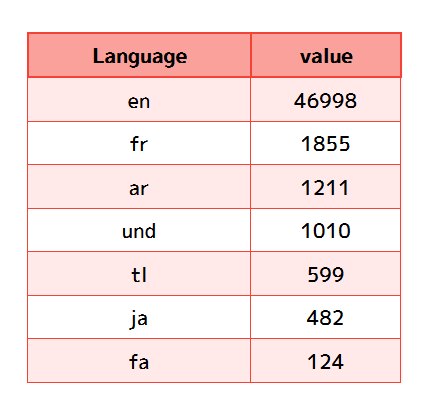
\includegraphics[scale=0.7]{diagrams/po_msf_lang.png}
    \caption{The graph show distribution of languages for a query \texttt{measles} in French, Arabic and English}
    \label{figure:msf_lang}
\end{figure}

The next occasion where Socneto proved itself was an analysis of trending topics of a convention Consumer Electronic Show (CES)\footnote{\url{https://www.ces.tech/}} that took place at the beginning of January 2020. Socneto helped to get a grasp of 120 thousand tweets during the three-day convention. The related topic analysis revealed that the most discussed topics were related to the television and car industry.

% no feedback will be present

% chronologický popis průběhu prací na projektu
% - Idea crystaliziation
% - First poc
% - Find real world users
% - finish
% - show
% - defend
% - party

\section{Project Timeline}\label{section:timeline}

The diagram of the project timeline is shown in Figure \ref{img:timeline}. The following text follows its structure.

\begin{figure}[h]
  \centering
    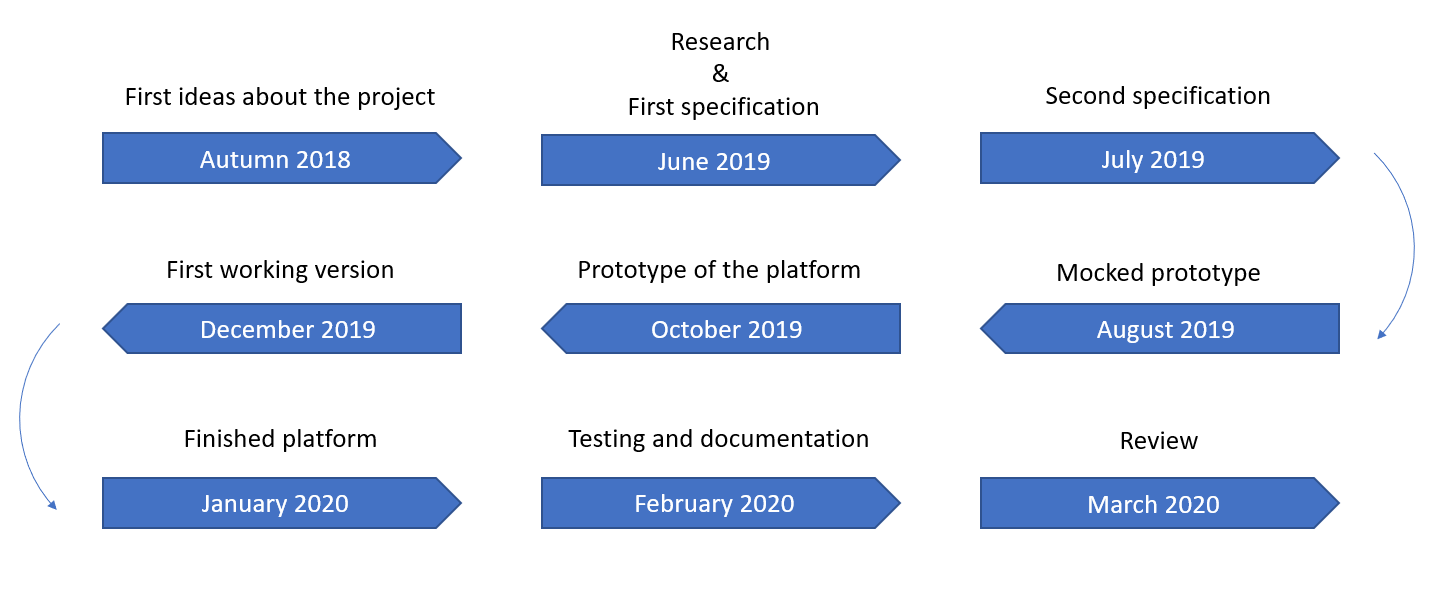
\includegraphics[width=\textwidth]{diagrams/timeline.png}
        \caption{Socneto development timeline showing the progress since Autumn 2018}
        \label{img:timeline}
\end{figure}

\subsection{Autumn 2018 - The First Idea}

The idea of creating a framework for data processing can be traced to Autumn 2018 and was motivated by the lack of practise with a big data framework. This idea was then consulted with the supervisor Doc. RNDr. Irena Holubová, Ph.D. who offered various feedback and helped us to find companies interested in cooperation. No cooperation was considered feasible though.  Soon after, Jan Pavlovský (a former member of the team) came up with an idea to focus on social network analysis. The idea seems to be interested enough for both parties and the search for the member started. Each member joining the team came up with ideas and the project started to take more solid shape. After many discussions, we came up with the idea of Socneto in June 2019 and the official project could start. 

\subsection{June 2019 - Official Start}
The software project work opened with writing the short specification with all the important ideas and features of the upcoming project. After it was accepted, the work on the second, full, specification could start. This document should contain not only a technical overview but also insight into project direction and management. We had an idea of separating the development into three stages: 
\begin{itemize}
    \item proof-of-concept - a project exploring the playing field, 
    \item full application - first application with all working components
    \item testing and documentation - last stage of the development
\end{itemize}

\subsection{July 2019 - Proof-of-Concept and Full Specification}

The proof of concept was finished along with the full specification in July 2019. At the time we were quite confident that we will not encounter any blind alley that would prevent us from finishing the project. Although most of the smart components were mocked, we found out that an application featuring an asynchronous messaging system would work. All mocked components were able to communicate well and others can be plugged in easily. 

\subsection{August 2019 to December 2019 - Working Prototype}

Most of our effort was put into replacing mocked components with working ones. Jaroslav Knotek finalized components downloading data from Twitter and Reddit. On top of that, we also added a component for the custom dataset which helped us with testing and at the end, it is a valuable addition to the offered ``data acquirers'' (for more information, see guide walking a user through the usage of custom dataset in Chapter \ref{chapter:extensibility}). 

Petra Vysušilová worked on sentiment analysis and topic modeling, replacing simple models with more elaborate ones. For better results, it was essential to get a more powerful infrastructure used for the training. For this purpose, the university GPU cluster was used to help train the model in a reasonable time. 

The entity model and all storage capabilities of Socneto were developed by Lukáš Kolek who built up storage for posts, their analysis, and all metadata. His part of Socneto, the whole database layer, is used by most of the components and is crucial for its proper function. Lukáš also helped to design interfaces between components so the communication would be as smooth as possible. 

The most visible part of the application was designed and implemented by Jůlius Flimmel who made it possible to visualize analyses and thus made them easily accessible. He was also responsible for designing the backend part of Socneto to ensure correct integration with the frontend.

This period was the time when Jan Pavlovský left the team after mutual agreement. Jan helped us the most at the beginning of the project when he proved to be a constant source of ideas. In the later phases, he has contributed to the architecture and a visual appearance. Unfortunately, his interest in the project was gradually diminishing after a discussion it was clear that did not intend to keep pace with the team. The project continued on with few changes. The support for the Czech language was omitted and all requirements concerning machine learning activities were lowered since Petra was the only remaining member capable of performing the task diligently.

\subsection{January 2020}

Because of a careful planning at the beginning, the implementation phase went smoothly without major hiccups. At the end of  December, we had a working platform with all the necessary components. It was time to find real-world users. With the help of Jiři Suchomel from the PR Department of the Faculty of Mathematics and Physics, we met Jan Böhm for whom we successfully analysed Twitter posts concerning measles and snake bites (for more details, see Section \ref{section:realuc}). 

\subsection{February 2020}
At the beginning of 2020 with the platform finished, we could start proper testing and documenting. At that time, we wrote scripts that start only a selected component in a controlled environment and assert its behaviour (see Chapter \ref{chapter:testing}). The documentation was written mostly during February. The 1st of March 2020 is the final deadline and according to the Software Project Committee customs we would be finished with defense by the end of the march. 
\chapter{Development Documentation}
\label{chapter:implementation}
\section{Architecture}

Socneto is a distributed application, the whole platform is robust and components are loosely coupled. Application is divided into services by their functionality. Everything is connected via Kafka messaging \ref{subsection:messaging} or internal REST API.

\subsection{Components}

Socneto is divided into eight logical parts:

\begin{itemize}
    \item Messaging (see Subsection \ref{subsection:messaging})
    \item Frontend (see Section \ref{section:frontend})
    \item Backend (see Section \ref{section:backend})
    \item Job managing service (see Section \ref{section:jms})
    \item Multiple data acquiring components (see Section \ref{section:acquirers})
    \item Multiple data analysers (see Section \ref{section:analysers}) 
    \item Storage (see Section \ref{section:storage})
    \item Monitoring (see Section \ref{section:monitoring})
\end{itemize}

Socneto can be extended by adding custom data acquirers or data analysers (for more details, see Section \ref{section:extensibility}). 

\subsection{Component Relationships}

The communication among the components respects the data flow of the application. A user submits a job through frontend to backend which notifies job management service (JMS). JMS then notifies all selected data acquirers and data analysers. The data analysers start to produce posts that start to flow into data analysers and to the storage. The analysers consume posts and produce analyses that are also sent to the storage. The storage consumes the posts and analyses and offers them to the user's queries through backend query endpoints. These relationships can be seen in Figure \ref{fig:concept}.

\begin{figure}[ht]
    \centering
    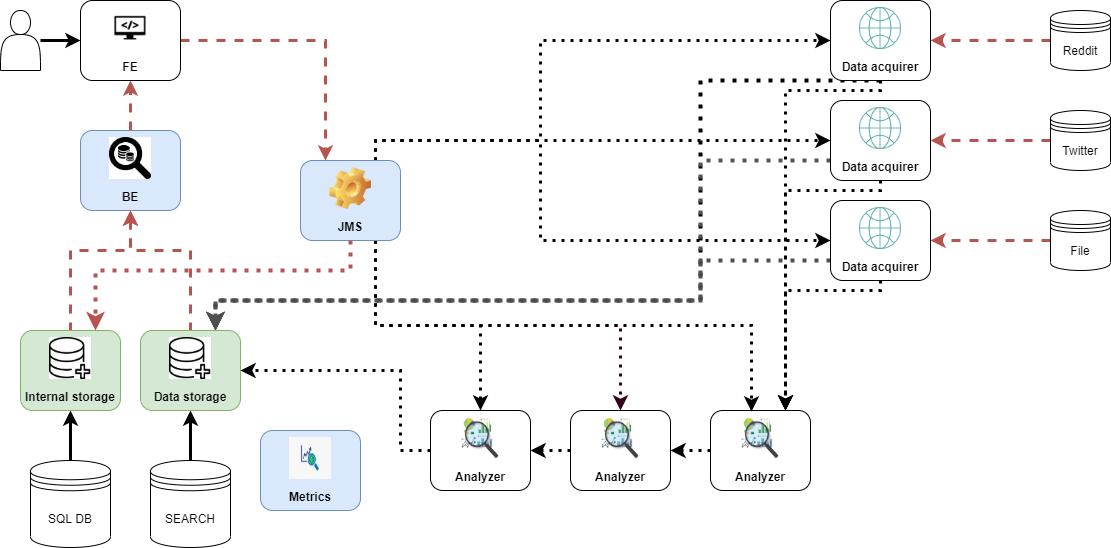
\includegraphics[width=\textwidth]{diagrams/soc-all.png}
        \caption{A diagram of the Socneto architecture showing relation ships among all components. This communication is asynchronous}
        \label{fig:concept}
\end{figure}

\subsection{Messaging}\label{subsection:messaging}

\paragraph{Publish \& Subscribe Principle}

\textit{"Publish/subscribe messaging, or pub/sub messaging, is a form of asynchronous service-to-service communication used in serverless and microservices architectures. In a pub/sub model, any message published to a topic is immediately received by all of the subscribers to the topic. Pub/sub messaging can be used to enable event-driven architectures, or to decouple applications in order to increase performance, reliability and scalability."}\footnote{\url{https://aws.amazon.com/pub-sub-messaging/}}

\paragraph{Publish/Subscribe in our Use-Case}

Posts are acquired and asynchronously sent to analysers and storage. Analysers subscribe to their assigned queues and after each analysis, they also send results to storage via messaging. Using this approach we achieved better extensibility of Socneto, high-throughput and loose coupling between modules. Defined message structures are described in Appendix \ref{appendix}. Acquirers and analysers get assigned topics during a registration and update processes.

\paragraph{Implementation}

In Socneto we have chosen Apache Kafka 2.4.0\footnote{\url{https://kafka.apache.org}} for messaging, which is an open-source project from Hadoop family\footnote{\url{https://hadoop.apache.org}} developed by Linkedin and the platform meets our requirements. Also, all common languages have a library with a connector to  Kafka.

\section{Project Structure}\label{section:projectStructure}

The project has the following directories
\begin{itemize}
    \item \texttt{acquisition} - Data acquirer code
    \item \texttt{analysers} - Data analyser code
    \item \texttt{backend} - Backend code
    \item \texttt{docs} - Documentation
    \item \texttt{frontend} - Frontend code
    \item \texttt{job-management} - Job Management Service code
    \item \texttt{storage} - Storage related code
    \item \texttt{tests} - Tests
\end{itemize}
\section{Frontend}\label{section:frontend}

Frontend enables the user to use the platform via a modern graphical interface. It is a web-based application, so it can be run in any environment with a web browser, however it is aimed for the environments with larger screens (i.e. computers, not phones). Using frontend, the user can:
\begin{itemize}
    \item \textbf{create jobs} - start acquiring and analyzing posts,
    \item \textbf{see the results} of jobs, including:
    \begin{itemize}
        \item \textit{analyses},
        \item optionally filtered acquired \textit{posts}
    \end{itemize}
\end{itemize}

\subsection{Dependencies}
Frontend requires \textit{\href{section:backend}{backend}} component to be running in order to function properly. This is caused by all the data it displays is being acquired via backend.

\subsection{Implementation}
The frontend is primarily written in \texttt{\href{https://angulardart.dev/}{AngularDart}} library \footnote{\url{https://angulardart.dev/}} with minority of the code being written in pure \texttt{JavaScript} and \texttt{CSS}. The \texttt{AngularDart} heavily uses \texttt{\href{https://dart-lang.github.io/angular\_components}{angular\_components}} library \footnote{\url{https://dart-lang.github.io/angularcomponents}}. It provides multiple reusable components which are based on \href{https://material.io/design/}{Material design} \footnote{\url{https://material.io/design/}}.

The whole frontend codebase can be found in \texttt{/frontend} directory of the project repository.

\subsubsection{Code - AngularDart}
As a typical Angular application, it uses \textit{component based architecture}. Each component consists of three parts:
\begin{itemize}
    \item \texttt{Dart} code - implements the business logic of the component (it is later compiled to \texttt{JavaScript}, which is described in Section \ref{section:frontend-build}),
    \item \texttt{HTML} code - a special version of HTML which supports interpolations of \texttt{Dart} code,
    \item \texttt{CSS} code - used for styling the resulting \texttt{HTML} code.
\end{itemize}
Each component is translated into an HTML tag.

The components are complemented with \textit{services}, which provide logic that is not bound to any component and \textit{models} which represent data and their structure.


\subsubsection{Services}
The logic which is used across multiple components, such as communication with backend, is implemented in services. These can be found in directory \texttt{/lib/src/services/}. Frontend contains the following services:

\begin{itemize}
    \item \texttt{HttpServiceBase} is an abstract wrapper of Dart's \texttt{\href{https://pub.dev/packages/http}{http package}}, which is implementation of HTTP protocol. This service adds an option to specify IP address and prefix of all HTTP requests. It also adds two functionalities to the http package:
    \begin{itemize}
        \item checking whether the HTTP response was successful (i.e. returned status code indicating success), or else throws \texttt{HttpException},
        \item deserializes and returns the JSON body of the response in form of Dart's Map object,
    \end{itemize}
    
    \item \texttt{HttpServiceBasicAuthBase} extends \texttt{HttpServiceBase} by adding \texttt{Autho\-rization} header to all HTTP requests using the \textit{basic authorization token}. This token can be specified directly, or by providing the service with username and password,
    
    \item \texttt{LocalStorageService} is a simple utility service which handles storing and loading of user credentials to the browser's local storage,
    
    \item \texttt{SocnetoDataService} extends \texttt{HttpServiceBasicAuthBase} with concrete HTTP requests to Socneto backend. All communication with backend is handled by this service,
    
    \item \texttt{SocnetoMockDataService} uses the same interface as \texttt{SocnetoDataService}, but instead of sending real requests to the backend, it returns mock data. This service should be used only during development and not on production!
    
    \item \texttt{SocnetoService} use \texttt{SocnetoDataService} via composition. It also uses \\ \texttt{LocalStorageService} to store and load user's credentials in the browser's local storage,
    
    \item \texttt{PlatformStatusService} is used to get the status of core Socneto components and inform subscribed Angular components about its changes. If any Angular component is subscribed for the changes, the service polls backend using \texttt{SocnetoService} every 5 seconds and asks about the platform status. If a different status is returned then in the previous request, then all the subscribed components are informed about this change.
    
\end{itemize}

\subsubsection{Components}
Most of the frontend codebase consists of implementations of multiple different components. These components can be found in directory \texttt{lib/src/components}. They are typically implemented in three parts (Dart, HTML and CASS). The convention in this project is, that each part is implemented in a different file. All of these three files are then placed in the same directory, have the same name and differ only in their extension. 

In this project, instead of using CSS, we use SCSS. Thanks to its more extensive syntax, SCSS is more user-friendly. However, it needs to be compiled later into CSS, because browsers do not support it. This process is described in Section \ref{section:frontend-build}.

Some components are designed for reuse in multiple other components. Their code is located in directory \texttt{lib/src/components/shared}. These components are:

\begin{itemize}
    \item \texttt{ComponentSelect} - gets a list of Socneto components on input and displays to the user the list of these components. The user can select any of these components, and after each selection change, this component triggers an event about it,
    
    \item \texttt{Paginator} is a simple visualisation of pagination. It displays a list of available pages and triggers an event on each page change,
    
    \item \texttt{PlatformStartupInfo} displays a warning for each core Socneto component which is not running. It subscribes itself to the \texttt{PlatformStatus\-Ser\-vice} to get notified on each component status changed. This component is used only during startup! After all  components are running, the component unsubscribes itself from the \texttt{PlatformStatusSer\-vice}, and will no longer show warnings if a component stops working,
    
    \item \texttt{SocnetoComponentStatus} - gets a \href{section:frontend-code-models-component-status}{\texttt{ComponentStatus}} as an input and displays it in a form of a colored icon,
    
    \item \texttt{Verification} is a modal dialogue, which is given a verification message on input, displays the message and triggers an event when the user presses the \texttt{yes} or \texttt{no} button.
\end{itemize}
The root component of the application, \texttt{App}, is the only direct child of HTML's \texttt{\textless body\textgreater} tag:

\begin{itemize}
    \item \texttt{App} is the root component of the application. Its only functionality is to check whether there are valid credentials in the browser's local storage and login the user automatically if there are,
    
    \item \texttt{AppLayout} is the only child of \texttt{App} component. It creates the main layout of the page:
    \begin{itemize}
        \item \textit{header bar} at the top of the page,
        \item \textit{hideable drawer} on the left,
        \item \textit{content} below the header. It can be either \texttt{Login} or \texttt{Workspace} component. Which of them is displayed is based on current page's URL\footnote{\url{https://angulardart.dev/tutorial/toh-pt5}}.
    \end{itemize} 
    
\end{itemize}
Description of other important components follows:

\begin{itemize}
    \item \texttt{Login} displays inputs for login and password. It also disables the inputs during the platform startup, while not all of the core Socneto components are not running,
    
    \item \texttt{Workspace} displays user's workspace when logged in. It is composed of two other components: \texttt{JobsList} on the left side and the second component on the right. The second component is chosen by current page's URL\footnote{\url{https://angulardart.dev/tutorial/toh-pt5}}. It can be either \texttt{QuickGuide} or \texttt{JobDetail} component,
    
    \item \texttt{JobsList} displays paginated list of all  user created jobs along with basic info about them. It is implemented using material list component\footnote{\url{https://dart-lang.github.io/angular\_components/\#/material\_list}}. The data for this component is retrieved from backend via \texttt{SocnetoService},
    
    \item \texttt{CreateJobModal} contains two-step material list component\footnote{\url{https://dart-lang.github.io/angular\_components/\#/material\_list}}. The first step contains inputs for each required field in a job definition and the second optional step contains credentials for the job. Only if a correct job definition is defined by the user, the job can be submitted to backend,
    
    \item \texttt{QuickGuide} displays a simple guide for the user. The guide is implemented using material stepper component \footnote{\url{https://dart-lang.github.io/angular_components/\#/material\_stepper}},
    
    \item \texttt{JobDetail} displays detail of the currently selected job in the \texttt{JobsList} component. It is a material list component with three tabs. The first tab contains \texttt{JobStats} component, the second contains \texttt{ChartsBoard} component and the third contains \texttt{PostsList} component,
    
    \item \texttt{JobStats} gets a \texttt{Job} on the input and displays some basic info about it and a few frequency charts (posts, language and author frequency),
    
    \item \texttt{ChartsBoard} gets a \texttt{jobId} on the input and displays one \texttt{Chart} component for each chart of that job. At the bottom of the list, it displays \texttt{CreateChartButton} component, which opens \texttt{CreateChartModal} when clicked on,
    
    \item \texttt{CreateChartModal} display inputs required for definition of a chart. Only a correct chart definition can be then submitted via backend,
    
    \item \texttt{Chart} get a \texttt{ChartDefinition} on input and queries chart data from backend according to it. It then displays the data in a chart. The chart's type is also selected from the chart definition,
    
    \item \texttt{PostsList} get \texttt{jobId} on input and displays \textit{paginated} list of posts acquired by the given job. The list is retrieved from backend. It also displays optional filters, which can be applied to the list. After each change in the filter, it queries backend for the posts again. It also contains a button to export all the (filtered) posts to CSV. The button's redirect URL is retrieved from backend.
\end{itemize}

\subsubsection{Routes}
Some of the components use angular routing\footnote{\url{https://angulardart.dev/tutorial/toh-pt5}} to select which component to display. All of the available routes are defined in \texttt{/lib/src/routes.dart}, along with their route parameters and mappings of concrete routes to concrete components.

\subsubsection{Styles}
Instead of using plain CSS, we use SCSS for its better and more extensive syntax.

The frontend uses two color palettes in each component - \textit{primary} and \textit{background}. In order to easily change these in the whole application, theming is implemented. Each component has its own styles wrapped in a SCSS mixin\footnote{\url{https://sass-lang.com/documentation/at-rules/mixin}}, which has a \textit{theme} parameter. This parameter contains both palettes, and every color used in the \textit{mixin} is picked from them. All  these component mixins are then included in the \texttt{apply-theme} mixin which passes the \textit{theme} parameter to each of them. We then implement multiple CSS classes which include this \texttt{apply-theme} mixin with different predefined theme objects, which can be found in \texttt{lib/src/style/theming/themes.scss}.

Different color palettes are defined in \newline\texttt{/lib/src/style/theming/palettes.scss}, which were created according to material color palette rules\footnote{\url{https://material.io/design/color/the-color-system.html\#color-usage-palettes}} using Palette Tool\footnote{\url{http://mcg.mbitson.com/\#!?mcgpalette0=\%233f51b5}}. The SCSS functions for retrieving specific colors from color palettes are implemented in \newline\texttt{/lib/src/style/theming/theming.scss}.

\subsubsection{Models}
Directory \texttt{/lib/src/models/} contains all of the models used throughout the application. It contains models for objects sent and received by backend as well as models used exclusively only on frontend. 

Models representing requests contain function \texttt{toMap()} which serializes them to Dart's generic \texttt{Map} object. This can be then easily serialized to JSON string by \texttt{HttpServiceBase} and sent to backend. 

Models representing responses from backend contain function \texttt{fromMap(Map data)}, which deserializes the \texttt{data} parameter into the model.

\subsubsection{Interoperability} \label{section:frontend-code-interoperability}
Dart SDK provides means to communicate with native JavaScript code via \texttt{js} package\footnote{\url{https://api.dart.dev/stable/2.7.1/dart-js/dart-js-library.html}}. This interoperability is required, when we want to use a \texttt{JavaScript} library, which was not rewritten to Dart. 

We use this functionality for two \texttt{JavaScript} libraries. One of them is \texttt{toastr}\footnote{\url{https://codeseven.github.io/toastr/}}, which is used to display notifications. The second one is Socneto's own JavaScript library for displaying charts. To be able to use these libraries, we implemented interfaces between Dart and them, using the mentioned \texttt{js} package. These interfaces can be found in directory \texttt{/src/lib/interop/}.

Even with these interfaces, we still need to import these \texttt{JavaScript} libraries from the resulting HTML code. This is done in \texttt{/web/index.html}. The \texttt{toastr} library requires \texttt{jQuery} library to function, so that one is also imported.

\subsubsection{Code - JavaScript}
To draw different types of charts, we use \texttt{d3js library}\footnote{\url{https://d3js.org/}}. This library was not rewritten to Dart. It also has an extensive API, so it would take considerable effort to create a Dart interface for it using Dart's \texttt{js} library as mentioned in Section \ref{section:frontend-code-interoperability}. For this reason, we  write chart components in pure JavaScript. From this code we then make a \texttt{JavaScript} library.

\texttt{Socneto} object implemented in \texttt{/lib/src/charts/charts.js} exposes multiple static functions for creating charts with data as their parameters. Implementations of the charts are then contained in separate JavaScript classes and CSS files located in the same directory.


\subsubsection{Static}
All the static image, which are used by the frontend are contained in \texttt{/lib/static} directory.

\subsubsection{Configuration}
\texttt{SocnetoDataService}'s backend address is read from environment variable \texttt{back\-endAddress}. It is read from the environment by utility class \texttt{Config}. If the variable is not specified, it defaults to \texttt{localhost:6010}.

The port where the frontend will be running is specified during build process (see Section \ref{section:frontend-build-no-docker}).

\subsubsection{Build and Run} \label{section:frontend-build}
The frontend can be built using two different methods. It can be built either by using Docker or without Docker.

\subsubsection {Build and Run - Without Docker}\label{section:frontend-build-no-docker}
To build the frontend without Docker, the following packages are required:
\begin{itemize}
    \item \textbf{Dart SDK} version 2.5.2 or higher,
    \item \textbf{NodeJs} version 8 or higher.
\end{itemize}
The following steps are required to build frontend:
\begin{itemize}
    \item \textbf{Gulp} - for better performance, we do not want to import from HTML all of our JavaScript and CSS files individually. To merge all of them into one JavaScript and one CSS file, we use \href{https://gulpjs.com/}{\textit{gulp} tool}. This tool can be installed only via \texttt{npm}, using command \texttt{npm install gulp \&\& npm install gulp -g \&\& npm install gulp-concat}. The gulp is configured via \texttt{/gulpfile.js} to do the merging as a default task. This means, we can run \texttt{gulp} command with no parameters or arguments and it will create the resulting two files, and put them to \texttt{/lib/static} directory.
    
    \item \textbf{Pub} - next, we need to download all the dependencies for our Dart application, which are specified in \texttt{/pubspec.yaml}. This is handled by running command \texttt{pub get},
    
    \item \textbf{Webdev} - the frontend server is started using \texttt{webdev} tool. This tool was already installed in previous step by \texttt{pub}. To be able to use the tool from command line, we need to activate it  using command \texttt{pub global activate webdev 2.5.1}. Now we can start the server using command \texttt{webdev serve}
\end{itemize}

\textbf{Note:} Since web browsers support only \texttt{CSS}, all of our \texttt{SCSS} files are compiled to \texttt{CSS} during the build. The compilation is done by \texttt{angular\_components} library, and it is specified in build configuration file located at path \texttt{/build.yaml}.

The resulting commands sequence is then following (run from \texttt{/frontend} directory of the Socneto repository):

\begin{lstlisting}[language=bash]
npm install gulp
npm install gulp -g
npm install gulp-concat
gulp
pub get
pub global activate webdev 2.5.1
webdev serve
\end{lstlisting}

Using \texttt{webdev serve} without any parameters, we start the server on address \texttt{localhost:8080} and compile Dart code to JavaScript using \texttt{dartdevc} compiler, which is more suitable for development then production. If we want to change the port, on which the server runs, we need to start it using command \texttt{webdev serve web:<PORT\_NUMBER>} (replace \texttt{<PORT\_NUMBER>}, with the required port number). If we are building the Dart web application on production, it is more suitable to use its \texttt{dart2js} Dart to JavaScript compiler. This compiler next to other features also minifies the resulting JavaScript, increasing the performance of our application. This can be achieved by running the above commands with option \texttt{--release}. 

\subsubsection {Build and Run - Using Docker}
To build the frontend using Docker, we need to have installed following pakcages:
\begin{itemize}
    \item \textbf{Docker} version 18.0.9.7 or higher.
\end{itemize}

The Socneto repository contains prepared functional \texttt{Dockerfile} located in directory \texttt{/frontend}. This \texttt{Dockerfile} builds the frontend using \texttt{dart2js} compiler (see Section \ref{section:frontend-build-no-docker}), and starts the server on port \texttt{8080}, accessible from \texttt{localhost} on host machine. To build and run the image, execute the following commands:

\begin{lstlisting}[language=bash]
docker build -t "frontend" .
docker run -p "8080:8080" "frontend"
\end{lstlisting}

After these commands the frontend can be accessed via a web browser on address \texttt{localhost:8080}.

\subsection{Communication}

Frontend communicates with Socneto via \href{section:backend-communication}{backend's HTTP JSON REST API}. 
\section{Backend}\label{section:backend}
Backend serves as a middle component between \textit{\hyperref[section:frontend]{frontend}} and the rest of the platform. It provides means for the users to retrieve different data from the platform and create new jobs. It also authenticates users using it and check whether the users are authorized to get the requested data.

\subsection{Requirements and Dependencies}
Backend requires two other components to be running in order to function properly:
\begin{itemize}
    \item \textbf{\href{section:jms}{Job Management Service}} - to create and stop jobs,
    \item \textbf{\href{section:storage}{Storage}} - to retrieve multiple different data.
\end{itemize}
It also needs Kafka for event tracking.

\subsection{Implementation} 
Backend is a web application running on ASP .NET Core 2.2 which implements standard Model-View-Controller principle. The solution follows data-driven-development which requires  the code base to be split into the following projects: 
\begin{itemize}
    \item \texttt{Api} - entry point of the application, contains configuration \texttt{appsettings.json} and controllers handling HTTP requests,
    \item \texttt{Domain} - business logic, platform independent,
    \item \texttt{Infrastructure} - platform dependent implementation.
\end{itemize}

The application uses dependency injection that is configured in the project \texttt{Api} in the file \texttt{Startup.cs}.

\subsubsection{Code}
The API's controllers are split according to which entities they operate with. Their role is to define concrete HTTP routes the API exposes, which HTTP methods they allow, and how the bodies of the requests look like. They also verify, whether the user querying the API is authenticated and authorized to do such requests. The authentication is implemented via HTTP's \texttt{Authorization} header, using \textit{Basic token}.

The following controllers are implemented:
\begin{itemize}
    \item \texttt{SocnetoController} is a base class for each controller. After handling each API request, it checks whether \texttt{ServiceUnavailableException} was thrown, and if it was, its sets the response's HTTP status code to 503 (Service unavailable),
    
    \item \texttt{ChartsController} defines API for management of charts. It defines requests for getting list of all charts defined for a job, creating a chart for a job and removing a chart from a job,
    
    \item \texttt{ComponentsController} defines API for listing components, which are connected to Socneto platform. It defines one route for getting all currently connected analysers and one for currently connected data acquirers,
    
    \item \texttt{JobController} defines API for retrieving job-specific data. It defines routes for listing all user's jobs, creating and stopping a user's job and getting status of a user's job. It also defines a route for getting posts acquired within a given job. The request is paginated and returns posts only from a given page and also support multiple filters. To get all the posts, it exposes another route, which returns all the posts in CSV formatted file. The controller also defines routes for retrieving aggregation and array type analyses for a given job, as well as basic analyses for each job, which are \textit{language frequency}, \textit{author frequency} and \textit{posts frequency},
    
    \item \texttt{ManagementController} defines API which informs whether the backend is running, and which other Socneto core components are running,
    
    \item \texttt{UserController} defines single API route, which is for logging in. It verifies, whether the user which is trying to login exists, and provided credentials are correct. 
\end{itemize}

The \texttt{Domain} project implements business logic of the backend. It is split into multiple services. While API project works only with interfaces of these services, their implementation are in this project. Just like the API project, Domain also defines multiple models, which define objects, that are transfered between backend and other Socneto components, or between API and Domain projects. 

The following services are implemented:
\begin{itemize}
    \item \texttt{AuthorizationService} implements the logic of verifying, whether a given user is able to interact with a given job in any way,
    
    \item \texttt{HttpService} is a wrapper over C\#'s \texttt{HttpClient}\footnote{\url{https://docs.microsoft.com/en-us/dotnet/api/system.net.http.httpclient?view=netcore-2.2}}. It implements utility functions for \texttt{Get}, \texttt{Post} and \texttt{Put} HTTP requests, which automatically check, whether the HTTP response was successful (HTTP status code which indicates success was returned), and deserializes the body of the response to a type specified by method's generic type. It also throws \texttt{ServiceUnavailableException} if the requested route is unavailable,
    
    \item \texttt{StorageService} implements Socneto's storage component REST API interface. All communication initiated by backend with storage component is handled by this service,

    \item \texttt{JobManagementService} implements Socneto's job management service's component REST API interface. All communication initiated by backend with JMS is handled by this service. It also sets default values for twitter and reddit credentials when submitting a job,

    \item \texttt{ChartsService} implements the logic behind creating, listing and removing charts for a given job. It queries storage component to retrieve and store the required data,
    
    \item \texttt{CsvService} implements creation of a CSV formatted file from a list of objects of the same serializable type. Serializable type in this context is a type, which uses \texttt{Newtonsoft.Json} library attributes, to mark, how it should be serialized into JSON. This service, however, uses these attributes to serialize the objects into CSV,
    
    \item \texttt{GetAnalysisService} implements creation and execution of correct queries to storage, to retrieve analysis of acquired posts with given parameters. A query creation is based on:
    \begin{itemize}
        \item \textit{Analyser's output format}: the query must ask for the field of the analysis, which is being populated,
        \item \textit{Type of the analysis}: the analysis can be an aggregation of analyses' field or an array of values of analyses' field,
        \item \textit{Requested result type}: the requested result may contain multiple analyses (e.g. line chart can contain multiple lines), in which case multiple queries to storage must be executed, and their results must be correctly merged together,
    \end{itemize}

    \item \texttt{JobService} implements retrieving jobs statuses and jobs' acquired posts from storage,
    
    \item \texttt{UserService} implements authenticating a user from given credentials. It queries storage whether the given user exists.
\end{itemize}

Event tracking is implemented by class \texttt{EventTracker}, which has public method for tracking messages on different levels (error, warn, info, ...). Any tracked message is enqueued to \texttt{EventQueue}. \texttt{EventSendingHostedService} then tries to dequeue a message from the \texttt{EventQueue} every 5 seconds and sends it via \texttt{IMessageBrokerProducer} to the platform.

The \texttt{Infrastructure} project implements functionality required by the chosen infrastructure of the platform. It contains implementation of \texttt{IMessageBro\-kerProducer} interface using Kafka.

\subsubsection{Configuration}
The configuration of backend is stored in project \texttt{API} in file \texttt{appsettings.json}. The configuration is distributed via a dependency injection  container. The most notable configuration objects are:
\begin{itemize}
    \item \texttt{KafkaOptions} - contains location of Kafka,
    \item \texttt{StorageOptions} - contains location of storage component's API,
    \item \texttt{JobManagementServiceOptions} - contains location of job management service component's API,
    \item \texttt{DefaultAcquirersCredentials} - contains default credentials for Twitter and Reddit acquirers, which are used if no credentials are specified via frontend when creating a job.
\end{itemize}

\subsubsection{Build and Run}
Backend can be built and run with two methods: with or without Docker.

If using docker, the required Docker version is \textit{18.0.9.7} or higher. The Dockerfile can be found in \texttt{/backend/} directory. From there, it can be built and run using the following commands:

\begin{lstlisting}
docker build -t "backend" .
docker run -p "6010:6010" "backend"
\end{lstlisting}
Then the backend's API can be found on \texttt{localhost:6010}.

If not using Docker, the project can be built and run using \textit{.NET Command Line Tools} (version 2.2.401 or higher). The following commands will build and start backend when executed from \texttt{/backend/Api}:

\begin{lstlisting}
dotnet restore # download all third party libraries
dotnet build # build the projects
dotnet run # run the project
\end{lstlisting}
After executing these commands, backend's API can be found on address\\ \texttt{localhost:5000}.


\subsection{Communication}\label{section:backend-communication}
Backend communicates with \textit{Storage} (Section \ref{section:storage}) and \textit{JMS} (Section \ref{section:jms}) components. It also exposes its own HTTP interface.

\subsubsection{HTTP interface}\label{section:backend-http-interface}
Backend exposes its own \textit{HTTP JSON REST API} for \textit{Frontend} to communicate with it. The API consists of multiple routes, which are documented in \texttt{/docs/api/be-api.pdf}.

\subsubsection{Outgoing communication}
To communicate with \textit{JMS} and \textit{Storage} backend uses their \textit{HTTP APIa} (see Sections \ref{subsubsection:jms_httpinterface} and \ref{subsection:storage-communication}).

Most of the requests on backend simply redirect them to one of the other two components with minimal changes and some input validation. 

\section{Job management service}\label{section:jms}

Job management service (JMS) responsibilities are:

\begin{itemize}
\item Keeping track of all registered components
\item Accepting submitted jobs
\item Distributing jobs among all components involved
\end{itemize}

\subsection{Requirements and Dependencies}

Job management service requires the following tools for it's proper function:

\begin{itemize}
    \item Kafka 2.4.0
    \item .Net Core 3.1.100
\end{itemize}

It communicates with the following service:
\begin{itemize}
    \item Storage service (see Section \ref{section:storage})
\end{itemize}

\subsection{Code}

JMS is web application running on ASP .NET Core 3.1 which implement standard Model-View-Controller principle. The solution follows domain-drive-principle\footnote{\url{https://docs.microsoft.com/en-us/dotnet/architecture/microservices/microservice-ddd-cqrs-patterns/ddd-oriented-microservice}} which requires  the code base into the following projects: 
\begin{itemize}
    \item \texttt{Api} - entry point of the application, contains configuration \texttt{appsettings.json} and controllers handling http requests
    \item \texttt{Domain} - business logic, platform independent
    \item \texttt{Infrastructure} - platform dependent implementation
    \item \texttt{Tests} - unit tests and integration tests
\end{itemize}

Application uses dependency injection that is configured in the project \texttt{Api} in the file  \texttt{JobManagementServiceBuilder.cs}.

JMS main domain is to manage jobs invoked via HTTP interface. Each job is performed by component. Since the components are not known in advance, each component needs to registered itself via Kafka interface. JMS is stateless, all the data is stored in storage service. The major components of JMS can bee seen in the Figure \ref{figure:class-jms}.
 
\paragraph{Major Classes}

\begin{itemize}
    \item \texttt{JobController} - The controller responsible for processing job related requests
    \item \texttt{SubscribedComponentManager} - Contains the vital logic of JMS implemented by the method \texttt{StartJobAsync}. Also used for registering components
    \item \texttt{RegistrationRequestListener} - Continuously listens to the topic\\ \texttt{job\_management.registration.request}. It is used by all other components to register themselves (for more details refer to Section \ref{subsubsection:jms_kafkainterface}). 
    \item \texttt{RegistrationRequestProcessor} - Parses registration requests and stores it in the database
    \item \texttt{StorageService} - Used as a proxy to storage service (see Section \ref{section:storage})
\end{itemize}

\begin{figure}
    \centering
    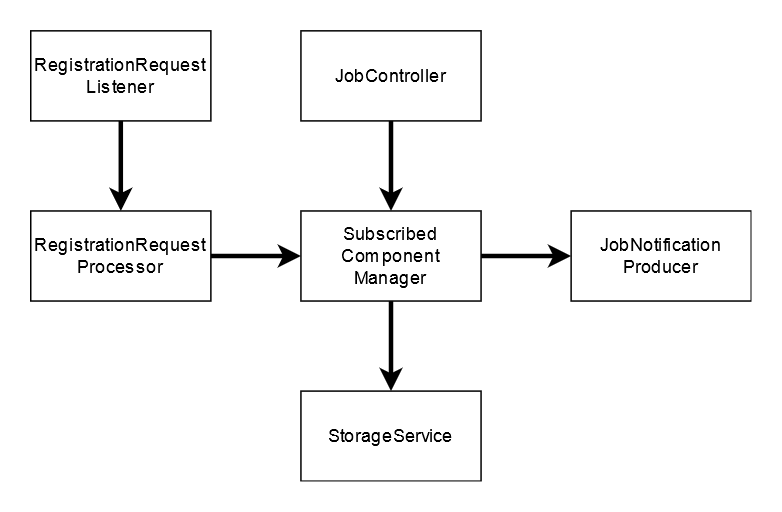
\includegraphics[width=0.9\textwidth]{diagrams/class-jms.png}
    \caption{The diagram shows relationships among major classes of JMS}
    \label{figure:class-jms}
\end{figure}

\subsection{Configuration}

The configuration of JMS is stored in the project \texttt{Api} in the file \texttt{appsettings.json}. It does not require any user's input. The configuration is distributed via a dependency injection container. Each option of the configuration needs to be bound to the file. This binding is in the project \texttt{Api} in the file  \texttt{JobManagementServiceBuilder.cs}.

The most notable configuration objects:

\begin{itemize}
    \item \texttt{KafkaOptions} - contains URI of Kafka. In case of starting JMS differently then advised, this element would need to be changed. (for \texttt{localhost} for example).
    \item \texttt{JobStorageOptions}, \texttt{StorageServiceHealtcheckOptions}, \texttt{Component\-StorageOptions} - these objects contain endpoint routes for the storage service. 
    \item \texttt{StorageChannelNames} - names of Kafka topics used to propagate posts and analyses to the storage.
\end{itemize}

\subsection{Build + Run}

Navigate to the source code, specifically to the \texttt{job-management/Api} type in the following commands:

\begin{itemize}
    \item \texttt{dotnet restore} - downloads all third party libraries
    \item \texttt{dotnet build} - build the projects
    \item \texttt{dotnet run} - run the projects
\end{itemize}

\subsection{Communication}\label{subsection:jms_communication}
\begin{figure}[H]
    \centering
    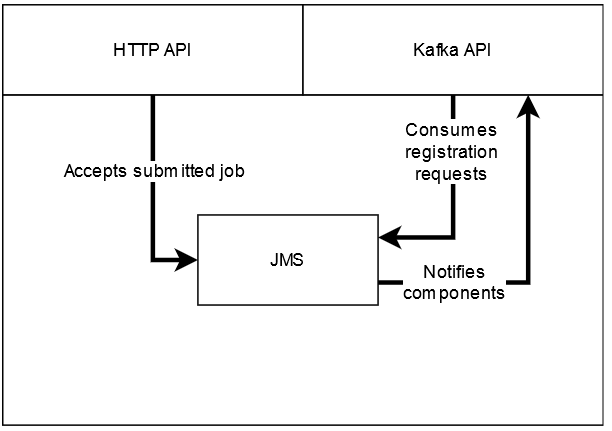
\includegraphics[width=0.8\textwidth]{diagrams/api-jms.png}
    \caption{HTTP interface is used to start or stop jobs. Kafka interface is used to listen to registration requests}
    \label{fig:apiJms}
\end{figure}
JMS uses Kafka and HTTP for communication depicted in Figure \ref{fig:apiJms}.



\subsubsection{Kafka Interface}\label{subsubsection:jms_kafkainterface}

Kafka is used to listen for registration request of the JSON format on the topic \texttt{job\_management.registration.request} from all components. 

The registration request (see Appendix \ref{subsection:registrationrequest}) of a component must contain the following fields:

\begin{itemize}
    \item \texttt{componentType} - either \texttt{DATA\_ACQUIER} or \texttt{DATA\_ANALYSER} depending on the type of the component.
    \item \texttt{componentId} - unique id of the component
    \item \texttt{inputChannelName} - name of the channel unique to the component. The component will use it for ingesting the data (in case of acquirer, this field is \texttt{null}.
    \item \texttt{updateChannelName} - name of the channel that the component uses for accepting job notifications.
    \item \texttt{attributes} - an object contains any other attributes
\end{itemize}

\subsubsection{HTTP Interface}\label{subsubsection:jms_httpinterface}

JMS offers two endpoints accepting POST requests:

\begin{itemize}
    \item \texttt{/api/job/submit} - starts jobs and notifies all components
    \item \texttt{/api/job/stop/<jobId>} - stops the jobs on all the components. Has no payload.
\end{itemize}

Submitting a job requires a body with the JSON payload with the following fields:

\begin{itemize}
    \item \texttt{selectedDataAnalysers} - component ids of all selected analysers. If any analyser has not been registered yet, the request fails.
    \item \texttt{selectedDataAcquirers} - same but with acquirers.
    \item \texttt{topicQuery} - topic of interest.
    \item \texttt{jobName} - human readable name.
    \item \texttt{attributes} - custom attributes of selected components. If user wants the component to receive some attributes, the JSON object with the attributes must be wrapped with an element with the component id. 
\end{itemize}

\subsubsection{Outgoing Communication}

JMS sends job notifications to the components via Kafka. Each registered component has a topic on which it listens to job configuration. When the job (see Section \ref{subsubsection:jms_httpinterface}) is submitted, all components involved are sent a job notification (see Appendix \ref{subsection:notification}). The components that re-register themselves receive all active job configurations. This prevents allow crashing components to continue on unfinished jobs.

\section{Data Acquirer}\label{section:acquirers}

Data acquirer is a component downloading data from a social network (or any other component). Some social networks with free API impose limits on the amount of data downloaded (e.g., for Twitter limits refer to \footnote{https://developer.twitter.com/en/docs/basics/rate-limits}). These limits are tackled by downloading data continuously not in  one batch. 

The posts may come in various languages but the analyses can usually work only with English. For this reason, analysers can optionally translate all acquired posts from any language to English.

\subsection{Requirements and Dependencies}

\noindent
Data acquirers require the following tools for its proper function:

\begin{itemize}
    \item Kafka 2.4.0
    \item .Net Core 3.1.100
    \item Minio 6.0.8
\end{itemize}

\noindent
They communicate with the following services:
\begin{itemize}
    \item Storage service (see Section \ref{section:storage})
    \item Job management service (see Section \ref{section:jms})
\end{itemize}

\noindent
And, the following libraries are referenced:

\begin{itemize}
    \item LinqToTwitter 5.0.0
    \item Reddit 1.3.4
    \item MinioClient 3.1.8
\end{itemize}

\subsection{Code}

Data acquirers are web applications running on ASP .NET Core 3.1 which implement standard Model-View-Controller principle. The solution follows domain-driven-development which requires the code based into the following projects: 
\begin{itemize}
    \item \texttt{WebApi.*} - For each data acquirer there is separete entrypoint web project with its own configuraiton file \texttt{appsettings.json}
    \item \texttt{Domain} - business logic, platform independent
    \item \texttt{Infrastructure} - platform dependent implementation. Contains specific implementation of each data acquirer's logic
    \item \texttt{Tests} - unit tests and integration tests
\end{itemize}

The majority of code base is shared among the three out-of-the box working acquirers: Twitter, Reddit and custom dataset loader. The differences are only in the entrypoint project \texttt{WebApi.*} which differently sets up dependency injection container. Otherwise all the code is the same.



Data acquirer code base consists of the following classes (their relationships are depicted in Figure \ref{figure:class-da}):

\begin{itemize}
    \item \texttt{RegistrationService} - Service sending registration on startup
    \item \texttt{JobConfigurationUpdateListener} - Listener that listens for job notification.
    \item \texttt{TranslationService} - Service that calls the Azure Text Translator API via HTTP.
    \item \texttt{JobManager} - Service that makes sure that the job is running and the posts are being correctly produced.
    \item Twitter: \begin{itemize}
        \item \texttt{TwitterBatchLoader} - Service that loads the data from the API.
        \item \texttt{TwitterContextProvider} - Creates context of the whole acquirer.
        \item \texttt{TwitterDataAcquirer} - Class responsible for orchestrating twitter batches and creating twitter context.
    \end{itemize}
    \item Reddit: \texttt{RedditDataAcquirer} - Service that loads data from the Reddit api.
    \item CustomDataset: \texttt{CustomDataAcquirer} - Service that connects to the Minio server and downloads given datasets.
\end{itemize}

\begin{figure}[H]
    \centering
    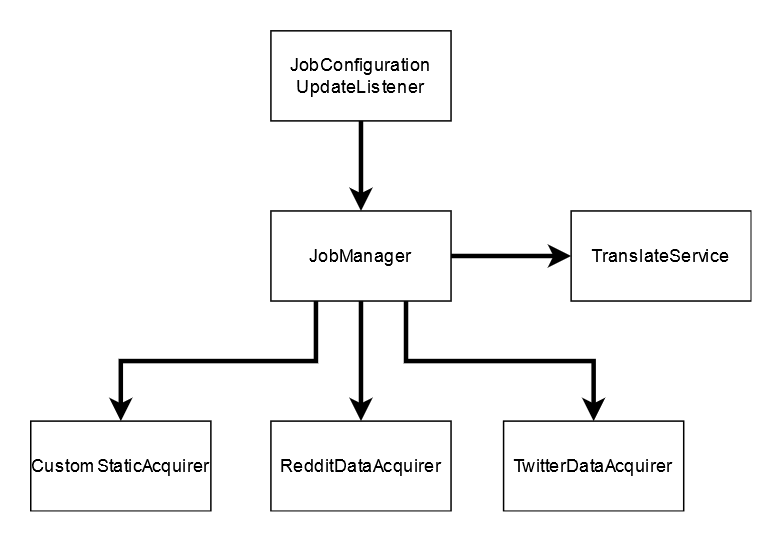
\includegraphics[width=0.8\textwidth]{diagrams/class-da.png}
    \caption{Relationships among major classes of Data acquirer}
    \label{figure:class-da}
\end{figure}

\subsection{Configuration}\label{subsubsection:acqconfig}

The configuration of an acquirer is stored in the project \texttt{WebApi.*} in the file \texttt{appsettings.json}. It does not require any user input. The configuration is distributed via a dependency injection container. Each option of the configuration needs to be bound to the file. This binding is in the project \texttt{Application} in the file \texttt{DataAcquisitionService\-WebApiBuilder.cs}.

\noindent
The most notable configuration objects are:

\begin{itemize}
    \item \texttt{ComponentOptions} - This object contains identity of the acquirer and Kafka topics which it uses.
    \item \texttt{TranslatorOptions} - This object contains settings of the translator service. Endpoint and subscription key can be found in a Azure Text Translator resource.
    \item \texttt{MinioOptions} - URL and credentials of the Minio server.
\end{itemize}

\subsection{Build + Run}

Navigate to the source code, specifically to the \texttt{acquisition/DataAcquirer/Web.*} and type in the following commands:

\begin{itemize}
    \item \texttt{dotnet restore} - downloads all third party libraries
    \item \texttt{dotnet build} - build the projects
    \item \texttt{dotnet run} - run the projects
\end{itemize}

\subsection{Communication}\label{subsection:da_communication}

JMS uses Kafka for the communication depicted in Figure \ref{fig:apiDa}

\begin{figure}[H]
    \centering
    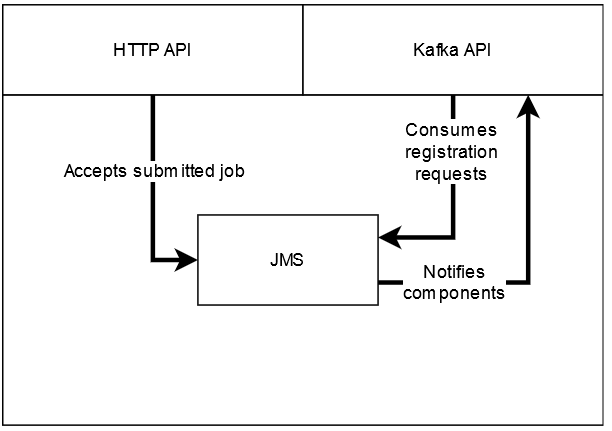
\includegraphics[width=0.8\textwidth]{diagrams/api-jms.png}
    \caption{Kafka interface is used to listen to job notification, produce posts and register the component}
    \label{fig:apiDa}
\end{figure}

\subsubsection{Kafka Interface}\label{subsubsection:da_kafkainterface}

Data acquirers listens for two types of job notification (see Appendix \ref{subsection:notification}): start job and stop job.

The start job notification has the following fields:

\begin{itemize}
    \item \texttt{jobId} - Id of the job
    \item \texttt{command} - In case of start job, it is always \texttt{START}
    \item \texttt{attributes} - attributes of the acquirer. It is discussed in more detail below.
    \item \texttt{outputChannelNames} - An array of topics that the acquirer produce posts into.
\end{itemize}

NOTE: The start notification is the same for analysers too.  
\\

Each acquirer requires different attributes:

\paragraph{Twitter Data Acquirer:}
\begin{itemize}
    \item \texttt{TopicQuery} - name of the topic
    \item \texttt{Translate} - is \texttt{"true"} when the post should be translated
    \item \texttt{ApiKey} - Api key used to identify application to the Twitter API.
    \item \texttt{ApiSecretKey} - Api secret  used to authenticate the application
    \item \texttt{AccessToken} - Access token issued by twitter application.
    \item \texttt{AccessTokenSecret} - Acess token secret used for authentication.
\end{itemize}{}

Example: 
\begin{lstlisting}[language=json,firstnumber=1]
{
  ...
  "attributes": {
    "TopicQuery":"weather pocasi",
    "Translate":"true",
    "ApiKey":"123erbs",
    "ApiSecret":"sdsfabnakaler"
    "AccessToken":"assadfsa23234dafadsfn1234123",
    "AccessTokenSecret":"ghfgdr4350234daf"
    }
}
\end{lstlisting}
The credentials showed do not represent valid credentials.

\paragraph{Reddit Data Acquirer}
\begin{itemize}
    \item \texttt{TopicQuery} - name of the topic
    \item \texttt{Translate} - is \texttt{"true"} when the post should be translated
    \item \texttt{appId} - Id of the application registered with twitter
    \item \texttt{appSecret} - Secret used to authorize the application.
    \item \texttt{refreshToken} - Token which is used to not let the session expire.
\end{itemize}{}

Example: 
\begin{lstlisting}[language=json,firstnumber=1]
{
  ...
  "attributes": {
    "TopicQuery":"weather;pocasi",
    "Translate":"true",
    "appId":"mffSocnetoApp",
    "appSecret":"adf289e8lmfals",
    "refreshToken":"klfoiowen1231"
    }
}
\end{lstlisting}
The credentials showed do not represent valid credentials.

\paragraph{Custom Static Data Acquirer:}
\begin{itemize}
    \item \texttt{Translate} - is \texttt{"true"} when the post should be translated
    \item \texttt{bucketName} - Name of the bucket in which is the custom data stored.
    \item \texttt{objectName} - Name of the dataset file
    \item \texttt{mappingName} - Name of the file with mapping
    
\end{itemize}{}

Example: 
\begin{lstlisting}[language=json,firstnumber=1]
{
  ...
  "attributes": {
    "Translate":"true",
    "bucketName":"example-dataset",
    "objectName":"myData.json",
    "mappingName":"myData.mapping"
    }
}
\end{lstlisting}

The stop job notification has the following fields:

\begin{itemize}
    \item \texttt{jobId} - Id of the job
    \item \texttt{command} - In case of stop job, it is always \texttt{Stop}
\end{itemize}

\subsubsection{Outgoing Communication}\label{section:da_outgoing}

\paragraph{Registration}
Acquirer needs to register itself on startup. The registration request was already discussed in the section JMS subsection Outgoing communication (see Section  \ref{subsubsection:jms_kafkainterface}).

\paragraph{Posts}

Data acquirer produces posts (see Appendix \ref{subsection:postmessage})  with the following fields:

\begin{itemize}
    \item \texttt{id} - Guid of the post
    \item \texttt{originalId} - Original id of the post issued by the respective social network.
    \item \texttt{jobId} - Id of the job in which context this post was produced
    \item \texttt{text} - Text of the post.
    \item \texttt{originalText} - If the translation is activated and the post was not originally in English, this field contains the original text and the field \texttt{text} contains the translation.
    \item \texttt{authorId} - Id of the author. In case of anonymous author,  value "0" is used.
    \item \texttt{language} - Language of the post in ISO 639-1 format.
    \item \texttt{datetime} - Datetime when to post was created conforming to format \texttt{YYYY-mm-DDTHH:MM:SS}.
\end{itemize}

The posts are typically produced to two channels: one that is consumed by the storage and the other consumed by all analysers since analysers produce only analyses, not the posts. These two entities are joined in the storage. Names of the channels are configurable and are discussed in the configuration part of Data acquirer (Section \ref{subsubsection:acqconfig}).

\section{Data Analysers}\label{section:analysers}

A data analyser is a component that consumes posts and produces per-post analysis. Socneto comes with two major analysis components: Topic modelling and Sentiment analysis. The implementation is common for both components. The functionality that is different is discussed in  Chapter \ref{chapter:analysis}.

\subsection{Requirements and Dependencies}

Data acquirers require the following tools for its proper function:

\begin{itemize}
    \item Kafka 2.4.0
    \item python 3.8
    \item Topic modelling trained model: en\_core\_web\_lg-2.2.5\footnote{\url{https://github.com/explosion/spacy-models/releases/download/en_core_web_lg-2.2.5/en_core_web_lg-2.2.5.tar.gz}} downloaded automatically upon building
    \item Trained sentiment model, also downloaded upon building.
\end{itemize}

They communicate with the following services:
\begin{itemize}
    \item Storage service (see Section \ref{section:storage})
    \item Job management service (see Section \ref{section:jms})
\end{itemize}

\subsection{Code}

The code wrapping libraries discussed in Chapter \ref{chapter:analysis} can be found in the \texttt{main.py} file. There are three notable functions:

\begin{itemize}
    \item \texttt{register\_itself} - sends registration requests (see Section \ref{subsection:registrationrequest}) whose attributes contains element \texttt{outputFormat} with the structure of format of the output analysis.
    \item \texttt{process\_acquired\_data} -  starts consuming topic where posts appear.
    \item \texttt{analyse} - invokes analysis.
\end{itemize}

\subsection{Build + Run}

\textbf{Topic modelling}:
\begin{itemize}
    \item \texttt{pip install -r requirements.txt} - installs requirements
    \item \texttt{wget -O en\_core\_web\_lg-2.2.5.tar.gz https://github.com/explosion/spacy-models/releases/download/en\_core\_web\_lg-2.2.5/en\_core\_web\_lg-2.2.5.tar.gz} - downloads the topic modelling trained model.
    \item \texttt{pip install en\_core\_web\_lg-2.2.5.tar.gz} - installs the model
    \item \texttt{python main.py}
\end{itemize}
 
\subsection{Configuration}

The script \texttt{main.py} accepts the following parameters:

\begin{itemize}
    \item \texttt{--server\_address} - address of the Kafka server
    \item \texttt{--input\_topic} - topic from which the analysers consume the posts.
    \item \texttt{--output\_topic} - topic to which the analysers produce analysis for the post (not the post itself). Set to the database input topic.
    \item \texttt{--registration\_topic} - topic to which the registration request is sent.
\end{itemize}

\subsection{Communication}\label{subsection:ds_communication}
\begin{figure}[H]
    \centering
    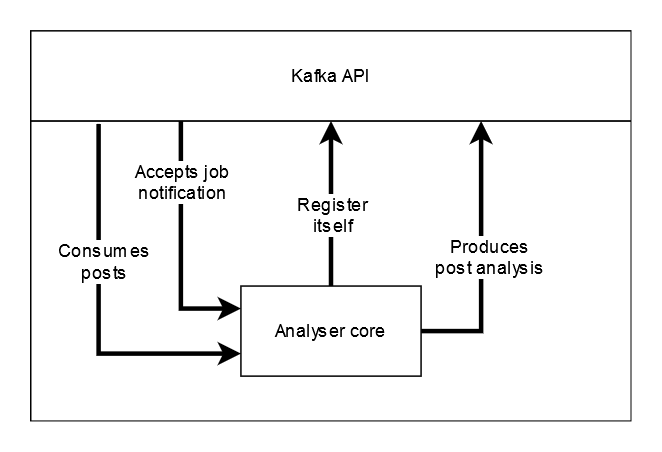
\includegraphics[width=0.8\textwidth]{diagrams/api-ds.png}
    \caption{Kafka interface is used to listen to job notification, produce analysis and register the component}
    \label{fig:apiDs}
\end{figure}
JMS uses Kafka for the communication depicted in Figure \ref{fig:apiDs}



\subsubsection{Kafka Interface}\label{subsubsection:ds_kafkainterface}

The simplicity of the analysers allows them to ignore job notifications. The only entity they consume is a post (see Appendix \ref{subsection:postmessage}) which has been already discussed in detail in Section \ref{section:da_outgoing}.

\subsubsection{Outgoing Communication}

\paragraph{Registration}\label{subsubsection:registration_analyser}

An analyser needs to register itself on startup. The registration request was already discussed in Section \ref{subsubsection:jms_kafkainterface}. The only addition is that they in element \texttt{outputFormat}.

\paragraph{Output format} Every analyser can produce any number of results, but the result value has to have one of the six possible formats:
\begin{itemize}
    \item \texttt{textValue} - a single string value
    \item \texttt{numberValue} - a single number value
    \item \texttt{textListValue} - a list of string values
    \item \texttt{numberListValue} - a list of number values
    \item \texttt{textMapValue} - a map of a string key and a string value
    \item \texttt{numberMapValue} - a map of a string key and a string value  
\end{itemize}
During registration each analyser has to pass a map with result name and its value type. This information is used during a chart definition on FE. The result has to be always in this format (see \ref{analysis} Analysis paragraph).

\paragraph{Analysis}\label{analysis}

Analysers produce analysis entity (see Appendix \ref{section:analysisMessage}) with the following fields:

\begin{itemize}
    \item \texttt{postId} - Guid of the related post
    \item \texttt{jobId} - Id of the job in which context this post was produced
    \item \texttt{componentId} - Analysers component Id
    \item \texttt{results} - Actual result of the analysis enclosed in an element with the analysis name.
\end{itemize}

\vspace{3\baselineskip}
Example - sentiment analysis: 

\begin{lstlisting}[language=json,firstnumber=1]
{
  "postId": "1234dsfgdsf",
  "jobId": "4df8165f-9461-4cdc-b6bc-b5fa0414319b",
  "componentId": "s_analyser_1",
  "results": {
    "polarity": {
        "numberValue": 1,
        "textValue": null,
        "numberListValue": null,
        "textListValue": null,
        "numberMapValue": null,
        "textMapValue": null
    }
  }
}
\end{lstlisting}
\newpage
Example - topic modelling: 

\begin{lstlisting}[language=json,firstnumber=1]
{
  "postId": "1234dsfgdsf",
  "jobId": "4df8165f-9461-4cdc-b6bc-b5fa0414319b",
  "componentId": "topic_analyser_1",
  "results": {
    "polarity": {
        "numberValue": null,
        "textValue": null,
        "numberListValue": null,
        "textListValue": ['food','bread',...],
        "numberMapValue": null,
        "textMapValue": null
    }
  }
}
\end{lstlisting}



\section{Storage}\label{section:storage}

Storage component is used for storing internal platform data, acquired posts and analyses. This module provides an abstraction of physical databases for the rest of the components. Every other component can communicate with the internal part of the storage via REST API and all internal entities support a custom subset of CRUD operations. Posts and analyses can be stored via messaging, but they can be queried only via REST API. This approach should help to increase the performance of the whole platform and loose coupling between components.

\subsection{Requirements and Dependencies}

Storage module needs a relational database for storing internal platform data, but posts and analyses must be stored in a storage, where it is easier to query those data, so the second storage dependency is a search engine.

\begin{itemize}
    \item Run: Java\footnote{\url{https://www.java.com/en/}}
        \begin{itemize}
            \item Minimal version of Java: 11
            \item Minimal version of Maven: 3.3.9\footnote{\url{https://maven.apache.org}}
        \end{itemize}
    \item Relation database: PostgreSQL\footnote{\url{https://www.postgresql.org}}
        \begin{itemize}
            \item Recommended version of PostgreSQL: 9.6
        \end{itemize}
    \item Search engine: Elasticsearch\footnote{\url{www.elastic.co/elasticsearch}}
        \begin{itemize}
            \item Recommended version of Elasticsearch: 7.4.2
        \end{itemize}
    \item Kafka broker
        \begin{itemize}
            \item Platform component
        \end{itemize}
    \item Messaging
        \begin{itemize}
            \item Platform component
        \end{itemize}
\end{itemize}

\subsection{Code}

For implementation Java 11 language with Spring Boot framework\footnote{\url{https://spring.io}} is used. Spring Boot framework was chosen due to easier and faster development, because it is built on the Inversion of Control principle\footnote{\url{https://en.wikipedia.org/wiki/Inversionofcontrol}} and also it provides an abstraction of databases and other dependencies. For building of the whole application multi-module Maven is used.

During the design phase, we included MongoDB\footnote{\url{https://www.mongodb.com}} as NoSQL database for posts and analyses. After some time we have not found any reasonable real-world use case for duplication of data. (Synchronization performance was not great and the storage was using more physical disc space than needed.) Also, Elasticsearch has made internal improvements, so it is more often used as primary storage. 

User authentication and authorization is not implemented in the current version of Socneto, because it is beyond its primary scope. If there is some identity provider in the future, it will be simple to improve security with Spring Security\footnote{\url{https://spring.io/projects/spring-security}}. As a temporal solution, users are imported into the database during the start of the application. This solution should only simulate user authentication. The correct solution is more complex, because it has to be reused in many components of the whole platform.

Storage component is divided into four modules. Every module has a different usage: storage of internal data, storage of posts and analyses, Kafka consumer and REST controllers. The main pattern besides IOC is used MVC with more layers: controllers, validation on data transfer objects, domain layer, persistence.


\paragraph{Module internal-storage}

This module can be used for CRUD operations with internal data (components, jobs, users, etc.). For storing data PostgreSQL is used and communication are done via Spring framework. The framework adds an abstraction of storage for this module.

\begin{itemize}
    \item Major classes:
        \begin{itemize}
            \item \texttt{ComponentDto} - description of Analyzer or Acquirer component
            \item \texttt{ComponentDtoService} - operations for \texttt{ComponentDto}
            \item \texttt{ComponentJobConfigDto} - configuration of components for a single job
            \item \texttt{ComponentJobConfigDtoService} - operations for \texttt{ComponentJobConfigDto}
            \item \texttt{ComponentJobMetadataDto} - object, where every component can store its metadata for a single job
            \item \texttt{ComponentJobMetadataDtoService} - operations for \texttt{ComponentJobMetadataDto}
            \item \texttt{JobViewDto} - view configuration of a single job 
            \item \texttt{JobViewDtoService} - operations for \texttt{JobViewDto}
            \item \texttt{UserDto} - internal user and password
            \item \texttt{UserDtoService} - operations for UserDto
        \end{itemize}
    \item App properties config:
        \begin{itemize}
            \item \texttt{spring.datasource.url} - JDBC string to database
            \item \texttt{spring.datasource.username} - database user
            \item \texttt{spring.datasource.password} - database password
        \end{itemize}
    \item Spring concept:
        \begin{itemize}
            \item Spring Boot Starter JDBC
        \end{itemize}
    \item Dependencies:
        \begin{itemize}
            \item PostgreSQL database
        \end{itemize}
\end{itemize}

\subsubsection{Module analysis-results}

Module analysis-results uses Elasticsearch for storing posts and analyses. These objects can be queried in many ways:

Posts support search queries with pagination and aggregations by authors, language, etc.

\begin{description}
    \item Query \texttt{POST\_AGGREGATION}:
    \begin{itemize}
        \item \texttt{COUNT\_PER\_TIME} - aggregation of posts over time
        \item \texttt{COUNT\_PER\_AUTHOR} - aggregation of posts per authors
        \item \texttt{COUNT\_PER\_LANGUAGE} - aggregation of posts per languages
    \end{itemize}
\end{description}

Analyses can be queried in a more complex way. The basic list with results can be queried with pagination, but also aggregation over list and map results is supported.

\begin{description}
    \item Query \texttt{AGGREGATION}:
    \begin{itemize}
        \item \texttt{MAP\_SUM} - sums occurences in \texttt{MapValue} result
        \item \texttt{LIST\_COUNT} - sums occurences in \texttt{ListValue} result
    \end{itemize}
    \item Query \texttt{LIST}:
    \begin{itemize}
        \item \texttt{LIST} - list of analyset result values
        \item \texttt{LIST\_WITH\_TIME} - list of analyset result values with time
    \end{itemize}
\end{description}

\begin{itemize}
    \item Major classes:
        \begin{itemize}
            \item \texttt{SearchPostDto} - an acquired post entity
            \item \texttt{SearchPostDtoService} - operations for SearchAnalysisDtoService
            \item \texttt{SearchAnalysisDto} - an analysis entity 
            \item \texttt{SearchAnalysisResultDto} - representation of analysis result value
            \item \texttt{SearchAnalysisDtoService} - operations for SearchAnalysisDtoService
            \item \texttt{ResultRequest} - a request for list values or agrregations
            \item \texttt{ResultService} - an aggregation service for posts and analyses
            \item \texttt{ListWithCount} - a result of list request with a total count filed
        \end{itemize}
    \item App properties config:
        \begin{itemize}
            \item \texttt{elasticsearch.host} - Elasticsearch host
            \item \texttt{elasticsearch.port} - Elasticsearch port
        \end{itemize}
    \item Spring concept:
        \begin{itemize}
            \item Spring Data Elasticsearch
        \end{itemize}
    \item Dependencies:
        \begin{itemize}
            \item Elasticsearch
        \end{itemize}
\end{itemize}

\subsubsection{Module storage-messaging}

This module is created for receiving posts and analysis messages from the Kafka message broker. Every message is parsed into an internal object and stored by the analysis-results module. The module consists of two configurable receivers for different topics.

\begin{itemize}
    \item Major classes:
        \begin{itemize}
            \item \texttt{AnalysisReceiver} - a consumer of analyses messages
            \item \texttt{PostReceiver} - a consumer of posts messages
            \item \texttt{KafkaConsumerConfig} - a consumer factory provider
        \end{itemize}
    \item App properties config:
        \begin{itemize}
            \item \texttt{spring.messaging.bootstrap-servers} - url to Kafka server
            \item \texttt{app.topic.toDbRaw} - a topic for post messages
            \item \texttt{app.topic.toDbAnalyzed} - a topic for analysis messages
        \end{itemize}
    \item Spring concept:
        \begin{itemize}
            \item Spring Kafka 
        \end{itemize}
    \item Dependencies:
        \begin{itemize}
            \item \texttt{analysis-results} module
            \item Kafka message broker
        \end{itemize}
\end{itemize}

\subsubsection{Module storage-web}

Storage-web module contains all REST endpoints of the storage component. It uses CRUD services from Internal-storage module and search services from Analysis-storage module.

Also, this module is the only one which can be run. For execution Spring Boot Starter is used, which starts all modules together, loads configuration, connects to Kafka, database, etc.

Validation of input API objects is done via \texttt{javax.*} annotations. This approach helps with validation without a huge amount of code and it is built on Spring framework.

\begin{itemize}
    \item Major classes:
        \begin{itemize}
            \item \texttt{ComponentController} - REST API for components
            \item \texttt{ComponentJobConfigController} - REST API for component job configs
            \item \texttt{ComponentJobMetadataController} - REST API for component job metadata
            \item \texttt{HealthCheckController} - health check endpoint
            \item \texttt{JobController} - REST API for jobs
            \item \texttt{JobViewController} - REST API for job view
            \item \texttt{PostController} - REST API for posts
            \item \texttt{ResultsController} - REST API for results
            \item \texttt{UserController} - REST API for users
        \end{itemize}
    \item App properties config:
        \begin{itemize}
            \item \texttt{app.componentId} - ID of Storage component
            \item \texttt{server.port} - Port of Storage component
        \end{itemize}
    \item Spring concept:
        \begin{itemize}
            \item Spring Boot Starter Web
        \end{itemize}
    \item Dependencies:
        \begin{itemize}
            \item \texttt{internal-storage}
            \item \texttt{analysis-results}
        \end{itemize}
\end{itemize}

\subsection{Build + Run}

\begin{itemize}
    \item Build: \texttt{maven package -f pom.xml}
    \item Run: \texttt{java -jar storage-web-1.0.0-SNAPSHOT.jar}
\end{itemize}

\subsection{Communication}\label{subsection:storage-communication}

The storage component provides two APIs. Kafka API is only for acquired posts and analyses. This API provides async communication for acquirers and analysers. For querying posts and analyses the REST API must be used. Both endpoints support pagination when it is needed. REST API is also used for CRUD operations of internal data. For better understanding, the flow is described in Diagram \ref{figure:storage}.

\begin{figure}[H]
\centering
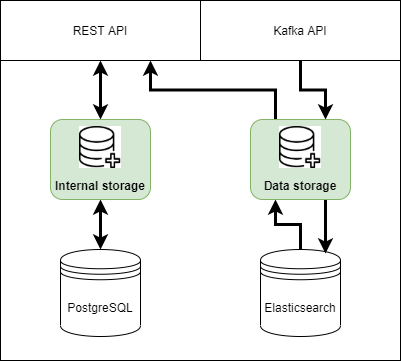
\includegraphics[width=8cm]{diagrams/socneto-storage.png}
\caption{Storage architecture uses two databases forming polyglot storage}
\label{figure:storage}
\end{figure}

\begin{itemize}
    \item REST
        \begin{itemize}
            \item Swagger: \texttt{$<$storage-host$>$:$<$storage-port$>$/swagger-ui.html}
            \item Exported swagger documentation: \texttt{docs/api/storage-api.pdf}
        \end{itemize}
    \item Messaging topics
        \begin{itemize}
            \item Posts:
            \texttt{job\_management.component\_data\_input.storage\_db}
            \item Analyses:
            \texttt{job\_management.component\_data\_analyzed\_input.storage\_db}
        \end{itemize}
\end{itemize}

\section{Monitoring}\label{section:monitoring}

The platform contains many components and, hence, a unified logging is useful when an application is deployed. ELK Stack\footnote{\url{https://www.elastic.co/what-is/elk-stack}} is used for platform monitoring purposes. Every component can log its events over HTTP (port: 9999) or through Kafka messaging (topic: log\_collector.system\_metrics) into Logstash\footnote{\url{https://www.elastic.co/logstash}}. Only Log entities (see Appendix \ref{section:logMessage}) with defined format must be used. When a log is received by Logstash, it is stored into Elasticsearch. (The platform uses the same instance for posts, analyses, and logs.) A user can open Kibana\footnote{\url{https://www.elastic.co/kibana}} dashboard in a browser and see logs from all components in one place. Architecture is described in Diagram \ref{figure:monitoring-diagram}.

\begin{figure}[H]
\centering
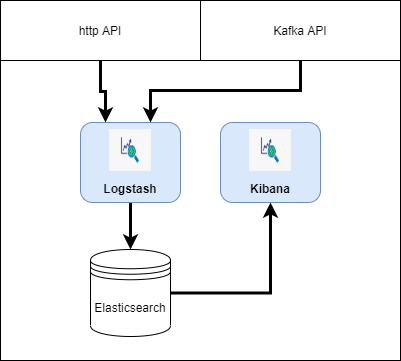
\includegraphics[width=8cm]{diagrams/socneto-metrics.png}
\caption{Diagram of monitoring interfaces. Logstash is connected to HTTP API and Kafka API and feed the data to database which is used by Kibana}
\label{figure:monitoring-diagram}
\end{figure}

\subsection{Requirements and Dependencies}

\begin{itemize}
    \item Logstash
        \begin{itemize}
            \item Minimal version of Logstash: 7.4.2
        \end{itemize}
    \item Kibana
        \begin{itemize}
            \item Recommended version of Kibana: 7.4.2
        \end{itemize}
    \item Elasticsearch
        \begin{itemize}
            \item Recommended version of Elasticsearch: 7.4.2
        \end{itemize}
    \item Kafka messaging
        \begin{itemize}
            \item Platform component
        \end{itemize}
\end{itemize}

\subsection{Configuration}

\subsubsection{Logstash Configuration}

\begin{lstlisting}[language=json,firstnumber=1]
input {
  http {
    id => "http_in"
    port => 9999
  }
  kafka {
    bootstrap_servers => "kafka:9092"
    topics => "log_collector.system_metrics"
    codec => "json"
  }
}

filter {
  if ![attributes] {
    mutate {
      remove_field => [ "attributes" ]
    }
  }
}

output {
  elasticsearch {
    hosts => [ "elasticsearch:9200" ]
  }
}
\end{lstlisting}

\subsubsection{Kibana Dashboard}

A user can specify his own dashboard with logs in Kibana. Possible fields are:
\begin{itemize}
    \item \texttt{componentId} - a name of a component
    \item \texttt{eventType} - FATAL, ERROR, WARN, INFO, METRIC
    \item \texttt{eventName} - a custom event name
    \item \texttt{message} - a custom message
    \item \texttt{timestamp} - a time when the log was created
    \item \texttt{attributes} - any JSON object with additional info
\end{itemize}
\section{Extensibility}\label{section:extensibility}

Socneto can be extended with custom data acquirers or data analysers. The components must implement the following stages properly.

\subsection{Contract}

\paragraph{Registration}
To component sends registration request (see Section \ref{subsubsection:jms_kafkainterface} to the topic \texttt{job\_management.registration.request} consumed by JMS (see Section \ref{section:jms}). This registration request makes the component discoverable. Without the registration, component could not be selected by the user. 

In case that the component was already registered and crashed. Upon the re registration, the component receives all the job notifications of running jobs that was received during the the component lifetime. This behaviour makes it easier for component to recover since it does not have to persist the notification itself. This behavior implies that the registration is idempotent therefore multiple re registration will not cause problems.

\paragraph{Starting a Job} 
After successful registration, the jobs notification (see Appendix \ref{subsection:notification}) starts flowing event to the channel specified in the \newline\texttt{updateChannelName} field in the registration request. The processing of those jobs has been already discussed in respective chapter of the analysing components (see Section \ref{subsubsection:ds_kafkainterface}) and data acquiring components (see Section \ref{subsubsection:da_kafkainterface}).

Data acquirers and data analysers react differently to the job notification. While data acquirers are expected to start producing posts (see Appendix \ref{subsection:postmessage}) to all topics present in the \texttt{outputChannelNames} array the acquirers need to wait for some posts from \texttt{inputChannelName} to come first then analyse them and produce the analysis (see Appendix \ref{section:analysisMessage}). In case of data acquirers, the job notification element \texttt{outputChannelNames} contain at least two topics: one represent a topic which storage consume to store raw posts. The others are then for each selected data analyser. In case of data analyser, the \texttt{outputChannelNames} is usually only one --- the storage input topic.

\paragraph{Stopping a Job}

The jobs can be stopped using also the job notification with a command element \texttt{command} set to \texttt{Stop}. This signals the component that can safely stop listening to the respective input topics. In case of analysers, stopping should be delayed for some time until the all of the messages are not consumed. Data acquirers should be shut down immediately.

\chapter{Text Analysis}\label{chapter:analysis}

\section{Introduction}
In this chapter, the social network posts text analyses originally featured in Socneto are described. 

The solved problems are presented in the section \ref{sec:posibilities} of this chapter. First, the motivation behind the choice of these problems and other possible types of analyses is discussed. Furthermore, a comparison of different input data types and their limitations is given. 
In the sections \ref{sec:topic_modelling} and \ref{sec:sentiment}, the chosen problems are described precisely together with selected solutions. A quick comparison of possible methods, the theory behind them and implementation details are provided for each problem.

Section \ref{sec:experiments} of this chapter is dedicated to a discussion of results and a conclusion.

\section{Natural Language Processing - Possibilities and Drawbacks}
\label{sec:posibilities}

As main goal of Socneto is analysis of posts from social networks, this section provides an introduction to a natural language processing (NLP). In Deep Learning book \cite{DeeplearningBook}, NLP is defined as \textit{"...the use of human languages, such as English or French, by a computer."}.

\subsection{What Is Possible}

The main intention of Socneto is to present automatically analysed data from various social networks. Socneto is extensible in many directions including new social networks and new types of analyses, but some analysis types are provided by default. Chapter \ref{chapter:implementation} of this documentation describe how to choose, obtain and store data from Reddit and Twitter. The question is, what to do with them. \par
NLP offers a variety of problems to solve. Some of them are  beyond our focus, for instance, conversion between written and oral language. We could imagine using this to analyse short videos published on Twitter. This could give us more text for analyses, but we  focus first on  basic analysis of the text we have.\par Another possible way of natural language processing is \textbf{syntax analysis} - examination of the formal structure of words, sentences and larger parts of the text. \textit{Sentence breaking} or \textit{word segmentation}, which divides the text into smaller, further analysed parts are included in the pipeline for text preprocessing. The task of \textit{lemmatization}, also used in preprocessing, lies in finding a base form of a given words, meaning for example nominative of singular for nouns or infinitive for verbs. The analysis can then continue with \textit{morphological segmentation}, which divides words into smaller parts, morphemes. To return to whole sentences, different types of trees are used to represent the structure of sentences and dependencies within a sentence (see Figure \ref{fig:trees}).
\begin{figure}[h]
\centering
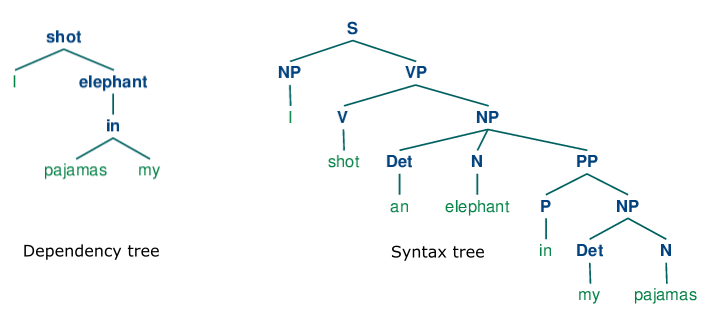
\includegraphics[width=1\textwidth]{diagrams/syntax_depedency_trees.png}
\caption{
An example of the syntax and dependency tree. Dependency tree, as the name indicates, describes dependencies between words. Such dependencies are of various types, for example an elephant in the example is an direct object of the shooting action. A root of such tree is typically a predicate of the sentence. On the other hand, syntax tree represents syntactic structure of the sentence according to the grammar. The root of the tree is \textit{sentence}, which is split to noun and verb phrase. These can be further divided into phrases compound from particular instances of parts of speech (e.g. nouns, adverbs, verbs, prepositions etc).
\newline \textit{Source: \cite{NLTKbook}}}
\label{fig:trees}
\end{figure}\par All previously mentioned treatments and many others are available for syntax analysis and most of them are needed for whatever task is performed, but they do not provide much information about the meaning of the text, at least for a human reader. \par More suitable for this purpose is the part of NLP dedicated to \textbf{semantic analysis}. Again, it contains various methods from natural language text generation to  recognition of homonymy or polysemy of given words. It could solve sophisticated assignments as answering questions about the input text document or  translation. Another possible task is to find in the text so-called named entities - like persons, months or cites - or linking these entities to some knowledge base. We can try to recognize the formality of the text, its sentiment, main topics or even try to automatically modify the text to be clearer. \par It is not necessary to be limited to text analysis only. In addition to speech recognition, it is also possible to engage in computer vision for extracting information from pictures. The importance of social networks data does not lie only in user contribution, but also in the metadata. Interesting results can be obtained via study of different user groups, their relationships to other groups, or different topics and opinions together with some demographic data.

\subsection{The Nature of the Data}
 Social networks have become important communication medium in recent times. They have the power to influence many people whether it is shopping, politics, environmental responsibility or the newest trends. So there are many reasons for understanding them. Data stored in networks are growing every second and it is not in human power to consume all of them. The problem of obtaining this data is solved by the acquiring mechanism of our platform as described in other sections of the documentation (chapter \ref{chapter:implementation}).
 \par
 Inputs to natural language processing can be data of many kinds. Both syntactic and semantic models can be trained on \textit{treebanks}. An example of a treebank is in Figure \ref{fig:pdt}). A treebank is a parsed corpus with various types of annotations.
For machine translation documents with many language versions are appropriate.

\begin{figure}
\centering
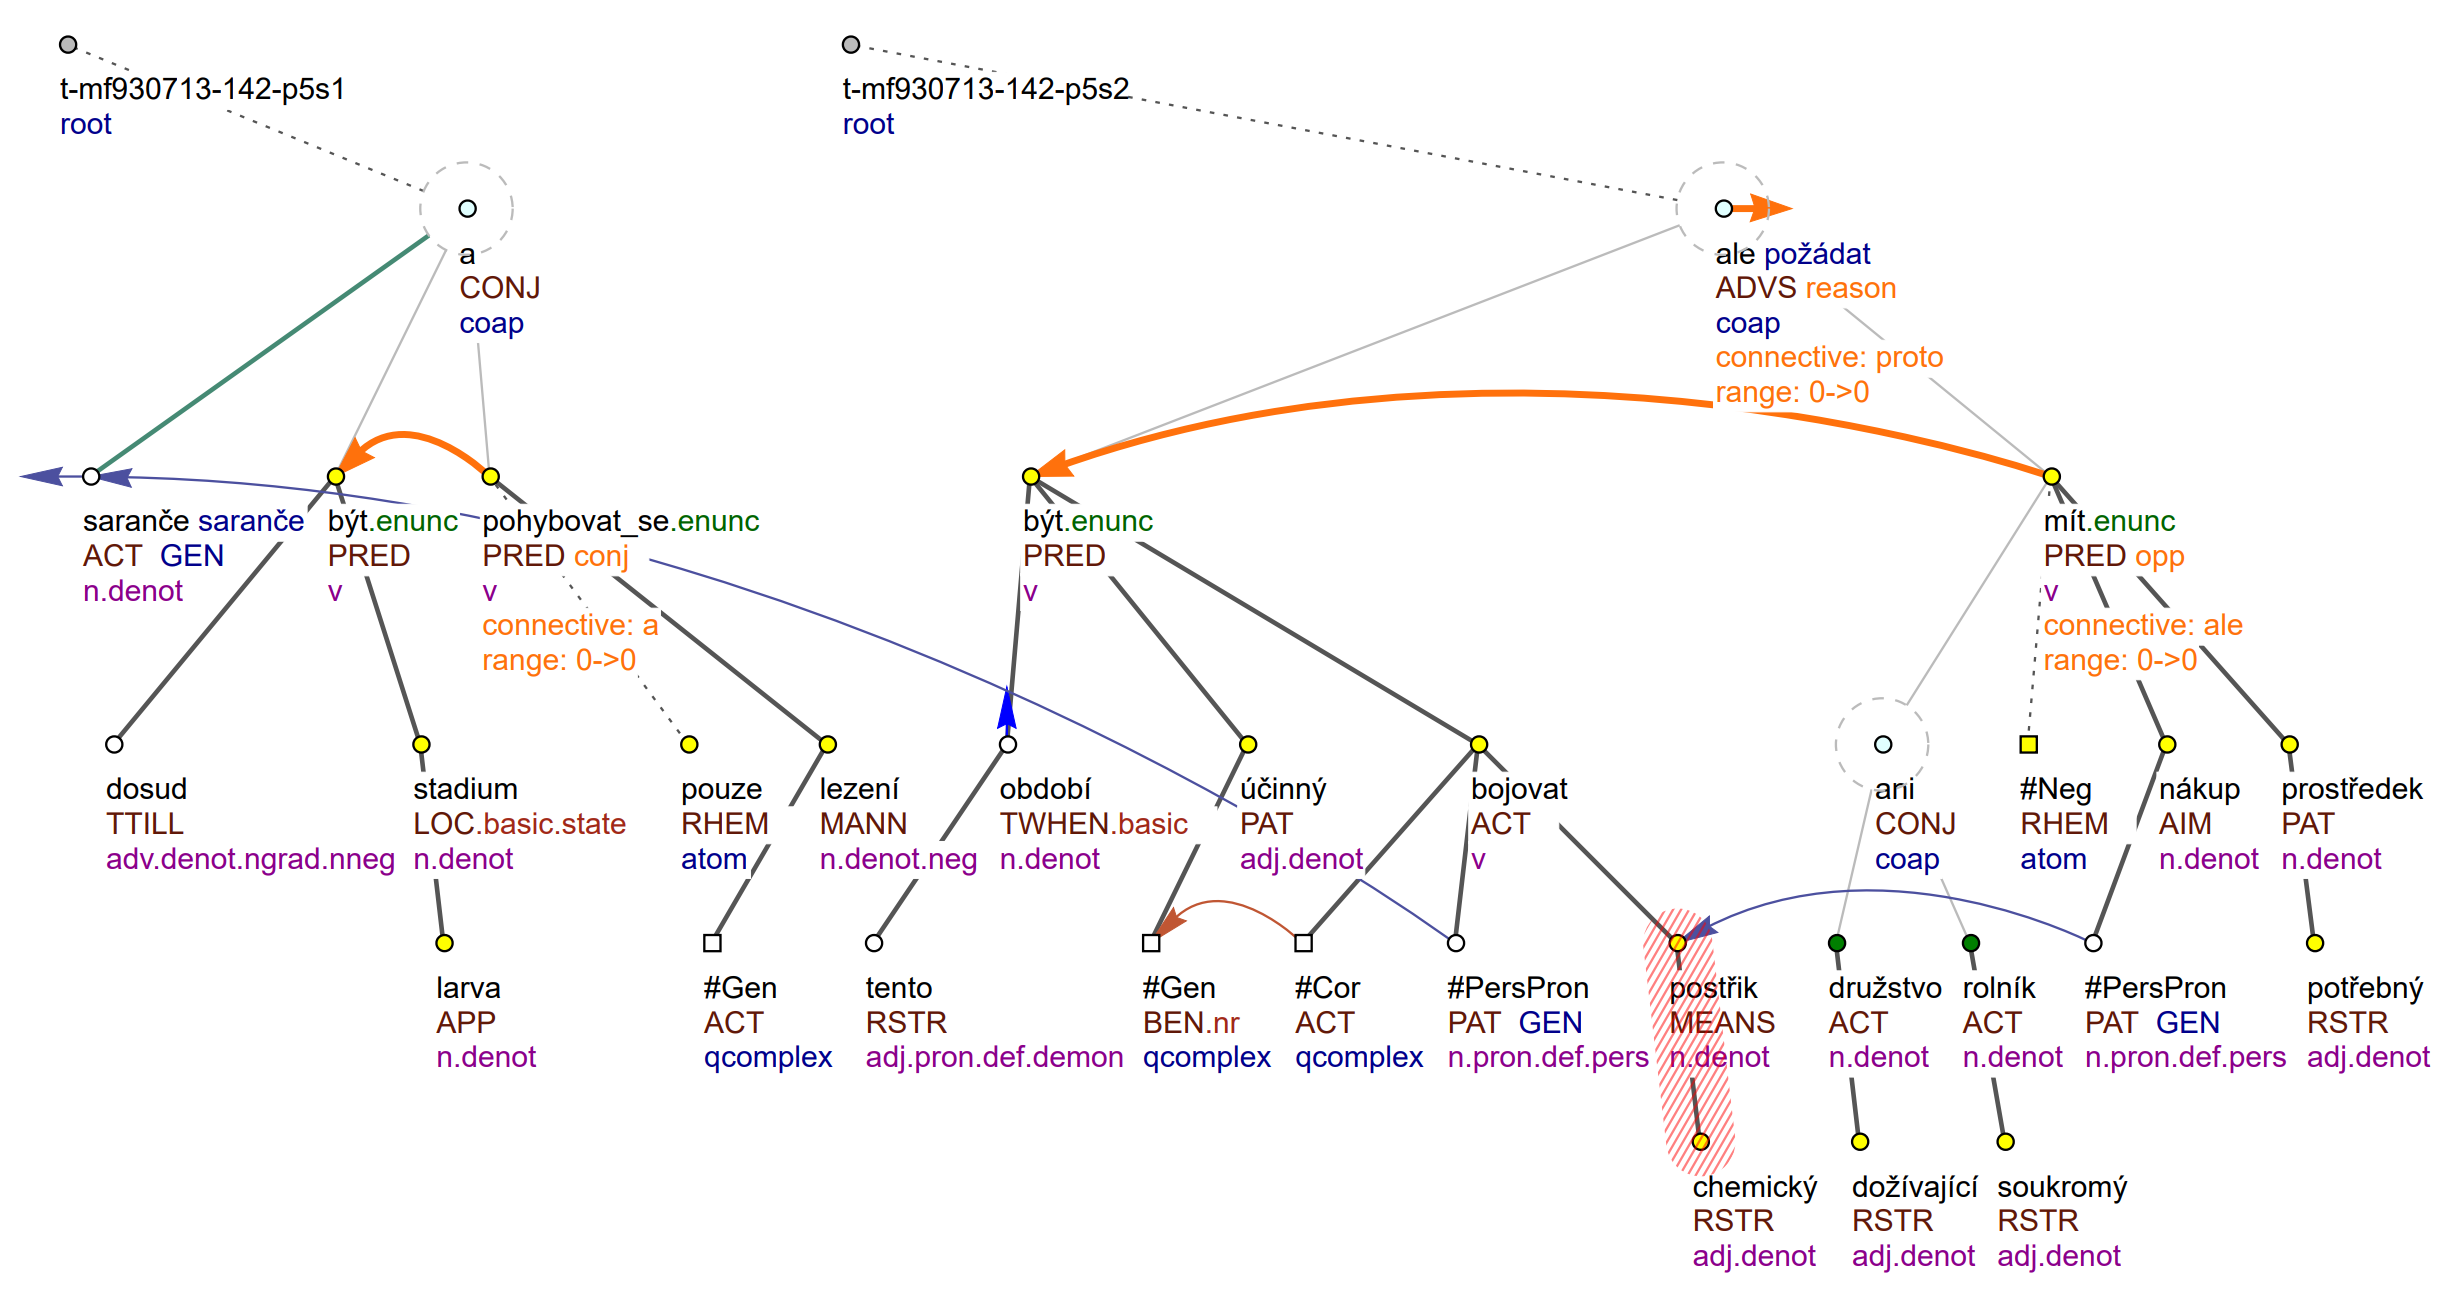
\includegraphics[width=1\textwidth]{diagrams/prague_dep_treebank.png}
\caption{
Prague dependency treebank example~\cite{PDT35} for the sentences: \textit{Sarančata jsou doposud ve stadiu larev a pohybují se pouze lezením. V tomto období je účinné bojovat proti nim chemickými postřiky, ale dožívající družstva ani soukromí rolníci nemají na jejich nákup potřebné prostředky}. This treebank contains dependency trees, but is is just one of many possibilities. This example is from Prague dependency treebank, which offers different layers of annotations. Red strips over words \textit{chemický} and \textit{postřik} marks multiword phrase, conjunction between \textit{rolník} and \textit{družstvo} is expressed as by one type of nodes, blue lines denotes coreference etc.}
\label{fig:pdt}
\end{figure}

Eurotra \cite{diane1995final} is, for example, almost twenty years lasting project of the European Commission dedicated to machine translation started on the latest seventieths. EU administrative documents in French and English served as datasets. \par
Topic modeling is typically applied on a big set of medium length documents (e.g.  scientific articles). In contrast, data from tweets and Reddit are different. Tweets are short snippets of text full of odd characters, newlines, and ends of lines. They contain pictures, emoji, a mixture of different languages, slang expressions, and grammatical errors. And they are very short, sometimes only one sentence long, few hashtags and a link or a picture.
Texts from Reddit are larger, but there is a challenging aspect of both social sites. The data has tree structure: Tweet and retweets or comments in the case of Twitter and main thread post with replies in the case of Reddit. These replies or comments can be even shorter than their parent post and/or do not mention previously said things explicitly. For performing a reasonable work of analysis it is necessary to have all these pieces of information together. \par Questions about the meaning of the text have another difficulty, which is, however, part of their attraction. They do not have always an unambiguous response. In the case of topic modeling, the goal is to identify general topics of a given text. These topics are not necessarily mentioned explicitly in the text and are then obviously hard to agree on them, especially if there is no given set of topics to choose from. Semantic analysis is a little bit easier. Evaluation of extremely positive or negative texts is mostly consistent among people. But of course, there is text somewhere in between, where classification is not so simple. Sentiment analysis must also deal with things like sarcasm or irony. It is not so complicated to learn a model when positive words like ``good'', ``nice'', ``favorite'' or ``love'' means positive sentiment of the classified text, but it is much harder to distinguish situations, where they mean the opposite.

The second problem connected with data quantity is a human inability to read them all. For this purpose, out-of-the-box analysis is aggregated to get a better overview. \par
\subsection{Choices for Socneto}
For these reasons we decided to focus on semantic types of analysis of data and to present two types of semantic analysis - \textit{sentiment analysis} and \textit{topic modeling}. Both these analyses helps us with extracting a meaning and their results can be aggregated in a reasonable way. Topic modeling allows us to identify popular topics themselves or to find other often related topics to the given one. So we can find out, what are people on social sites talking about. The second provided analysis - \textit{sentiment analysis} gives us an overview of their opinion about those topics. Both types of analysis are applied to a big bunch of data and return summary analysis, which is another useful feature. There are typically too many user posts to analyse, so inspecting each of them separately would produce an overwhelming amount of information and this does not solve the need for automatic analysis. 

\subsection{Machine Learning}

As in almost every machine learning application, possible methods can be supervised or unsupervised. Supervised methods require a dataset (sometimes called gold data), where  examples are problem instances together with correct answers. The learning algorithm then tries to find patterns or rules for classification and (iteratively) compares its answers with the correct ones. On the contrary, we need no correct answers for unsupervised learning. It is typically based on searching in the space of parameters to minimize some function (\textit{loss function)}. And it is also possible to solve tasks without machine learning at all by creating a set of hand-made rules. This approach is historically the first, but certainly not in the results.
\section{Topic Modeling (TM)}
\label{sec:topic_modelling}
Topic modeling task can be described by one of the following definitions:
\par
\begin{enumerate}

  \item A classification of a bunch of documents into a given number of topics together with learning typical keywords for each topic.
  \begin{itemize}
      \item \textbf{Input:} A set of documents, desired number of topics (integer, greater than zero).
      \item \textbf{Output:} Estimated probability distribution of topics for each document, estimated probability distribution of words for each topic.
    \end{itemize}
  \item Finding a list of words (=topics) associated with given data and their importance or distribution (which is what Socneto wants to do). 
  \begin{itemize}
      \item \textbf{Input:} Text for analysis (all tweets or posts together.)
      \item \textbf{Output:} A set of words best representing input.
    \end{itemize}

As there exists solution for the problem A, there also exists solution for problem B. It is true, because problem B can be transferred to the problem A by setting a count of topics to 1 and searching only for keywords. This does not solve the problem of finding abstraction topics not mentioned in the text but gives a quite good overview of the input data.
  \item A classification of texts into given topics.
   \begin{itemize}
      \item \textbf{Input:} Texts for classification, topics to choose from
      \item \textbf{Output:} One label from given topics for each text.
    \end{itemize}

\end{enumerate}
\subsection{Methods}
Regarding supervised methods, it is possible to use any known supervised classification algorithm. Among others support vector machines, logistic regression or neural networks belong here. The intended usage of Socneto is an application on data from many different areas, so we cannot define topics in advance, which is the reason, why our problem is not following definition C. \par This determines us to use unsupervised methods. For TM defined as in definition A, two mainly used methods are Latent Semantic Analysis (LSA) \cite{LSA} and Latent Dirichlet Allocation (LDA) \cite{LDA}. They are both based on the same assumptions, but LDA is an improved version of LSA with better performance. Topic modeling as in definition B was chosen for implementation, so we use LDA for it. A detailed description of theory and implementation is available in the following section. \par
Because LDA used in the described way (i.e. following the definition B) can find only words explicitly expressed in the text, we wanted to enrich the analysis by some more abstract topics. It can be done via solving \textit{entity linking} problem, which assigns hierarchical structure of categories to found entities/topics. The structure for classification is called the knowledge base and can be extracted automatically for example from Wikipedia. Or we can solve another problem - \textit{Named Entity Recognition} (NER). Algorithms for NER are able to tag each named entity by its category. Categories vary depending on implementation and training data, but categories like city, proper name, date, language or month can occur. This is supervised learning, but with a limited quantity of target classes and allows us to search for topics in specific categories provided by NER.
\par

\subsection{NER}
The task of finding named entities in the text and classifying them into the right category.
   \begin{itemize}
      \item \textbf{Input:} Unstructured text (= natural language), categories
      \item \textbf{Output:} Classification into right category if exists for all words (see Figure \ref{fig:NER})
    \end{itemize}
    
NER can be divided into two subtasks - identification of entities and their classification. As for every classification task, we can use supervised machine learning or rule-based system written by an expert. Another useful feature of this analysis is to recognize not only words but whole phrases (e.g.  National Park). This analysis can served as another tool for exploring the data. It allows filtering topics by categories like \textit{person} or \textit{place}. It can also helps to improve topic searching, as named entities are typically important int the text and NER is able to find pronoun references to them. Without such references, the word can occur just for one time and could appear as unimportant to LDA.

\begin{figure}[h]
\centering
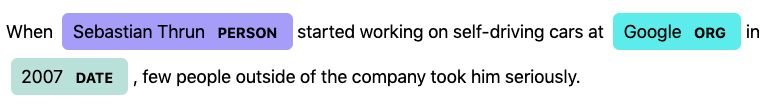
\includegraphics[width=1\textwidth]{diagrams/NER.png}
\caption{
An output of the Named Entity Recognition. Example from the SpaCy library documentation}
\label{fig:NER}
\end{figure}
Our analysis provides classification into 18 classes (see Table \ref{tab:nerclasses}) as we used third-party library SpaCy\footnote{\url{www.spacy.io}}, where these classes are predefined. 

\begin{table}[h]
\centering
\footnotesize
\begin{tabular}{ l p{0.7\textwidth} }
\hline
  \textbf{Class} & \textbf{Description} \\ \hline \hline
  PERSON & People, including fictional. \\ \hline
 NORP &  Nationalities or religious or political groups. \\ \hline
 FAC &  Buildings, airports, highways, bridges, etc. \\ \hline
 ORG &  Companies, agencies, institutions, etc.\\ \hline
 GPE &  Countries, cities, states.\\ \hline
 LOC &  Non-GPE locations, mountain ranges, bodies of water.\\ \hline
 PRODUCT &  Objects, vehicles, foods, etc. (Not services.)\\ \hline
 EVENT &  Named hurricanes, battles, wars, sports events, etc.\\ \hline
 WORK\_OF\_ART &  Titles of books, songs, etc.\\ \hline
 LAW &  Named documents made into laws.\\ \hline
 LANGUAGE &  Any named language.\\ \hline
 DATE &  Absolute or relative dates or periods.\\ \hline
 TIME &  Times smaller than a day.\\ \hline
 PERCENT &  Percentage, including "\%". \\ \hline
 MONEY &  Monetary values, including unit.\\ \hline
 QUANTITY &  Measurements, as of weight or distance.\\ \hline
 ORDINAL &  “first”, “second”, etc.\\ \hline
 CARDINAL &  Numerals that do not fall under another type.\\ \hline
 \end{tabular}
\caption{Classes in NER (spaCy)}
\label{tab:nerclasses}
\end{table}

 \par The used library, SpaCy, has pre-trained models for tagging and entity recognition for different languages. Algorithms in this library are not exactly based on one article, that could be named. Based on the GitHub discussion \cite{NERSpacy}, spaCy implementation of NER can be shortly described as classification using Convolutional Neural Networks (CNN) as in paper \cite{NERpaper}, but residual connections are used instead of dilatation and there are some other minor differences. Together with residual connections, there are two other important features - word embedding strategy using subword features and a transition-based approach. All three principles will be shortly described now. 
 \subsubsection{Word Embeddings with Subwords}
 Word embeddings are numbers or numerical vectors representing some categorical features. Their interesting feature is that when the source categories are near to each other, their embeddings are as well. Each dimension of the vector represents a different property of the word. One famous example for all: Embedding for the word 'Queen' can be almost exactly computed by the following formula on respective embeddings
 $king - man + woman$. A limitation of the original paper on embeddings \cite{mikolov2013efficient} concept was its inability to represent the morphological structure of the word. Embeddings were created based on the corpus and their occurrence in a similar context. It means, that no embedding exists for a newly seen word, even if it is morphologically very similar to a known one. Numeric representation of n-gram taken into account during the computation of an embedding is a solution to the problem.\cite{ngram_embedd}
 After this step, all words are represented by their embeddings and the following processing is performed only on them. 
 \subsubsection{CNN with Residual Connections}
 The convolutional neural network (see Chapter 9 in \cite{DeeplearningBook}) is a type of deep neural network with good ability to represent structures in the space. The input of this network is not a vector but a matrix (like a picture represented by values of its pixels). There is one single path from the input to the output of the network and every layer consists in the application of a filter or multiplication by a kernel on the sliding window.
 \par
In the case of residual connections, the network is split into smaller parts. To avoid  vanishing of information during the flow through the network, new shortcut connections (= residual connections) are added between some nodes. This approach is widely used in image recognition but also spread to other fields (see Figure \ref{fig:resnet}).
\begin{figure}[h]
\centering
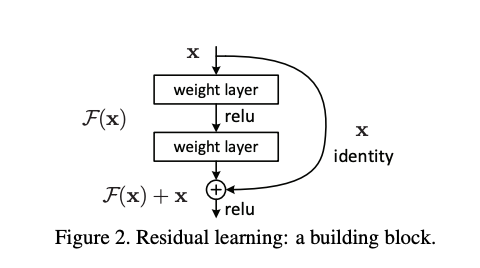
\includegraphics[width=0.7\textwidth]{diagrams/residual_connection.png}
\caption{
An example of the network for image recognition with residual connections. Residual network is a chain of layers with connections between as in deep forward networks, but there is also added connection marked as x identity, because in this case the activation function on the residual is identity function, which creates shortcut for strengthening information flow through the network.
\textit{source: \cite{DBLP}}}
\label{fig:resnet}
\end{figure}

\subsubsection{Transition Based Approach}
This approach consists of a sequence of small steps. In every step, only one word from the buffer is labeled or just one change to the configuration is applied \cite{daume2006practical}.

\subsection{LDA}
%co chceme, co je vstup a vystup, jak se to da udelat 
As mentioned above, Socneto uses LDA in the following manner:
   \begin{itemize}
      \item \textbf{Input:} A list of words (extracted from the text)
      \item \textbf{Output:} Top $n$ (in our case $n=10$, but it can be changed) words describing input.
    \end{itemize}
As the data are full of odd characters, newlines, and ends of lines, the first step is to clean the data. Our first trials have shown that adjectives are rarely useful, even indeed they make results messy and not informative at all. The same applies to pronouns, so words of both categories are removed. We can do this because the input of LDA is just a list of words, thus we can remove those words we don't want to be considered. We use the same pipeline described in the section \ref{sec:implementTM} because it helps us with the filtration. \par
%Now is time for the description of the theory. 
The previously mentioned LSA is an ancestor of LDA and it is better for showing basic ideas behind these two methods. LSA (same as LDA) is based on two assumptions: 
\begin{itemize}
  \item Every document contains a mixture of topics.
  \item Every topic is connected with different, but not necessarily disjoint, set of words. 
\end{itemize}
LSA than creates a matrix of documents contra terms, where values are \textit{tf\_idf}-s, where \textit{tf} stands for a term frequency
\[ tf = \frac{term\_occurences}{number\_of\_words\_in\_document} \]
and this is count over the whole corpus of documents (do not forget, that LSA is primarily applied on the corpus of different documents), while \textit{idf} is inverse document frequency
\[\frac{number\_of\_documents}{number\_of\_documents\_with\_term}.\]\textit{Idf} works as an evaluation of the importance of the word. The result is then: \[tf\_idf = tf \cdot idf .\] This matrix is then decomposed using \textit{singular value decomposition} (SVD). Decomposition gives us three matrices - $S$, $U$ and $V$. Matrix $S$ is always diagonal and each element on the diagonal represents one topic. Matrices $U$ and $V$ are document-topic and term-topic matrices respectively (see Figure \ref{fig:svd}) and they contains probability distributions. 

\begin{figure}[ht]
\centering
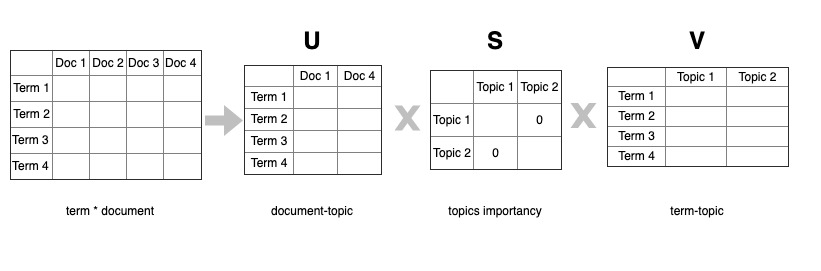
\includegraphics[width=1\textwidth]{diagrams/LSA.jpg}
\caption{
LSA matrix decomposition.}
\label{fig:svd}
\end{figure}
Selected $k$ greatest elements of $S$, corresponding columns from $U$ and rows from $V$ gives us k most important topics. $V$ than offers most important words for given topics.\par
LDA is based on the same assumptions. Unlike LSA, LDA assumes that topics and words follow Dirichlet's distribution. LDA tries to learn a model that best explains how data was generated.
\subsection{Implementation}
\label{sec:implementTM}
LDA model is created using package Gensim\footnote{\url{www.radimrehurek.com/genisim}} built by NLP Centre of the Masaryk University \cite{nlpcentre} especially for topic modeling, which pratically the only possible solution. We considered two libraries for NER task - \textit{NLTK}\footnote{\url{www.nltk.org}} and \textit{spaCy}. As using spaCy is much more comfortable than NLTK, we chose spaCy. Besides, SpaCy also seems to have superior performance on Twitter-like data \cite{TwitterNerComparison} (see Table \ref{tab:nerComparison}). These two considered libraries are not state-of-the-art possibilities, but provide reasonable results. The performance can be improved by using for example Standford CoreNLP, which is more technically demanding, but offers better precision. Socneto, though, expects human receiving result and than recall is maybe more importnant metric than precision, as mentioned also in \cite{TwitterNerComparison}. It is better to see all results and discard some wrongly classified than miss some results.

\begin{table}[h]
\footnotesize
%\begin{tabular}{@{}llll@{}}
\begin{tabular}{llll}
\textbf{System Name}                & \textbf{Precision}  & \textbf{Recall}   & \textbf{F1 Score}  \\
Stanford CoreNLP              & 0.526600541 & 0.453416149 & 0.487275761 \\
Stanford CoreNLP (with Twitter POS tagger) & 0.526600541 & 0.453416149 & 0.487275761 \\
TwitterNER                 & 0.661496966 & 0.380822981 & 0.483370288 \\
OSU NLP                  & 0.524096386 & 0.405279503 & 0.45709282 \\
Stanford CoreNLP (with caseless models)  & 0.547077922 & 0.392468944 & 0.457052441 \\
Stanford CoreNLP (with truecasing)     & 0.413084823 & 0.421583851 & 0.417291066 \\
MITIE                   & 0.322916667 & 0.457298137 & 0.378534704 \\
spaCy                   & 0.278140062 & 0.380822981 & 0.321481239 \\
Polyglot                  & 0.273080661 & 0.327251553 & 0.297722055 \\
NLTK                    & 0.149006623 & 0.331909938 & 0.205677171 \\ 
\end{tabular}
\caption{Comparison of available NER models for Twitter data. Data comes from Workshop on Noisy User-generated text \cite{wnut} 2016. \newline \textit{source: \cite{TwitterNerComparison}}}
\label{tab:nerComparison}
\end{table}

SpaCy, in addition, offers a built-in preprocessing pipeline, which we  used in both LDA and NER. Such a pipeline aims to transform the raw text into something more organized. In the case of spaCy, it contains a tokenizer, tagger, parser and named entity recognizer (see Figure \ref{fig:pipeline}), where:
\begin{itemize}
  \item Tokenizer: Breaks the full text into individual tokens.
\item Tagger: Tags each token with part-of-speech tag as noun, pronoun, adjective, punctuation etc. \cite{tags},
\item Parser: Creates syntactic tree, finds noun phrases.
\item Named Entity Recognizer (NER): Labels named entities.
\end{itemize}
\begin{figure}[H]
\centering
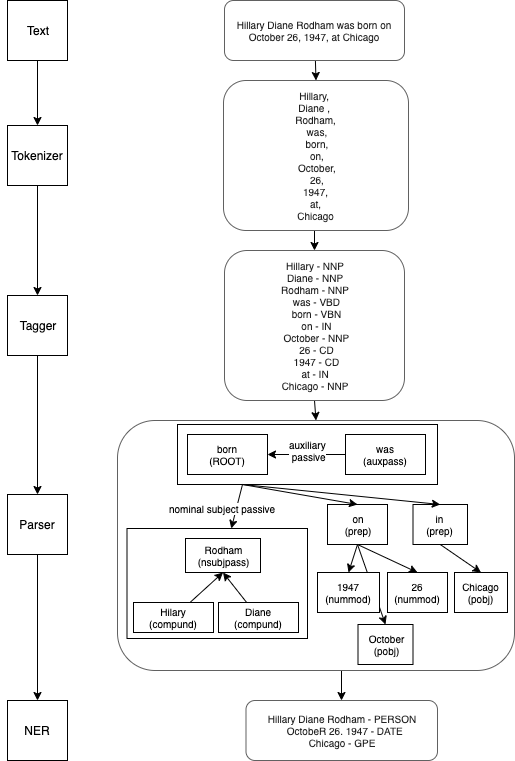
\includegraphics[width=0.7\textwidth]{diagrams/PIPELINE.png}
\caption{An example of processing in SpaCy pipeline.}
\label{fig:pipeline}
\end{figure}

\section{Sentiment Analysis (SA)}
\label{sec:sentiment}
We will consider the sentiment analysis task in the following form:
\begin{itemize}
    \item \textbf{Input:} A snippet of text (article, tweet etc.)
    \item \textbf{Output:} Classification into one of classes - positive, neutral, negative. 
\end{itemize}

Sometimes there is also considered so-called \textit{subjectivity} \cite{veselovska-2017}. It tries to classify if the opinion (both positive or negative) is objective or the author is personally interested and has strong emotions about his claims. For example, the following text could be recognized as objective: ``The sound of this notebook is clear.'', ``The base is not stable enough.'' or ``An internet connection in this area is bad.'' in contrast with ``I hate the way the new touchpad works.''. The subjectivity of the claim does not depend on its sentiment.
This part of sentiment analysis was not included in our project yet, but it is one of the possible extensions.
\subsection{Methods}
According to NLP-progress page \cite{sotasentiment}, actual state-of-the-art accuracy of this task on English datasets in the case of binary classification is above 95\%. Our demands, however, are higher than just binary classification. Classifying into more classes is noticeably harder, so our expectations about model performance are lower. As in the case of the TM task, some gold data labels could be subject to dispute, but it is still easier to classify into one of three given categories. \par
The chosen methods for this type of analysis are the Bidirectional Encoder Representations from Transformers (BERT) . The first idea of BERT was published in the first half of 2019 by Google AI Language \cite{bert} and since then, it is a leading approach to various NLP tasks. Not only that its results in many tasks are new state-of-the-art numbers, but its main advantage is a universality and easy use for different types of prediction. This allows distribution of non-specific pre-trained models, while fine tuning on any task could be done just by adding one simple layer on the top. This practice, known as \textit{transfer learning} has a long history in image processing. Unlike previous widely used models, BERT model just represents some universal knowledge about language. The next section is devoted to the further explanation of BERT ideas.
\subsection{BERT}
BERT model is built upon the idea of \textit{transformers}. A transformer is a neural network with two parts - encoder and decoder. Contrary to other types of neural networks, the input of a transformer is the whole sentence of text. Inputs are fed to the network in the form of embeddings, and the transformer tries to learn how to encode the sentence in the way that decoder can reproduce the original sentence. The whole training is an oscillation between decoder learning the best way to decode encoder output and encoder trying to learn better representation for the given sentence. In BERT, only the encoder is used. BERT model has three main features to describe - usage of embeddings, masked language modeling (MLM) and next sentence prediction. Each of them is described in the following text.
\subsubsection{Embeddings}
Following the transformers paper \cite{vaswani1706attention},
inputs are transformed into three types of embeddings: token embeddings, sentence embeddings and special transformer positional embeddings (see Figure \ref{fig:bert_emb}). These embeddings serve as a technical simplification for other model parts.

\begin{figure}[H]
\centering
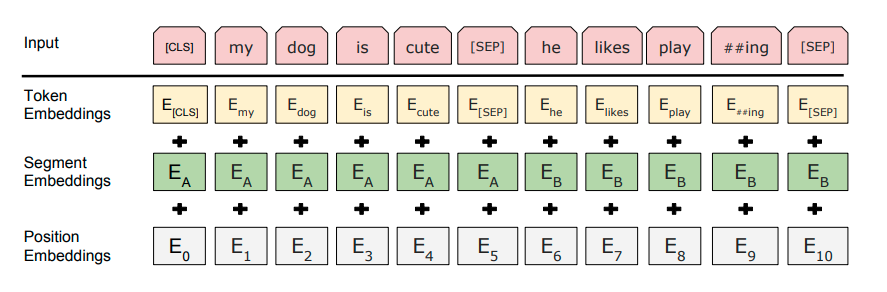
\includegraphics[width=1\textwidth]{diagrams/BERT-emb.png}
\caption{
Structure of BERT input embeddings. Input is enriched of tokens for start and end of sentences and then represented by embeddings for each word (token embeddings), embeddings for sentence (segment embeddings, same for words in one sentence) and position embeddings (position of token in the text).
\textit{source: \cite{bert}}}
\label{fig:bert_emb}
\end{figure}

\subsubsection{MLM}
MLM is a method for learning the language model. 15\% of input words are masked. Some of them will be visible at the end, but most of that, 12\%, is replaced by token [MASK].
This way the model improves the prediction of masked words based on the surrounding context.
\subsubsection{Next Sentence Prediction (NSP)}
NSP is a similar concept to MLM. In one part of the training, inputs of the model are pairs of sentences. In 50\% cases, the second sentence follows the first one in the training data. Otherwise, the second member of the pair is a random sentence from the data. The model then learns how to predict the following sentence.

\subsubsection{Whole Model}
MLM and NSP are combined and reflected in the loss function. The resulting language model is not trained to perform a specific task and this is done by stacking one or more layers at the top of this model. Then it is possible to combine training of these new layers only with allowing the gradient to flow through all model layers.

\subsection{Implementation}
The main third-party implementation to use for BERT is transformers by HuggingFace \cite{Wolf2019HuggingFacesTS}.
This library contains implementations of recent state-of-the-art ideas including BERT and its variations together with a pre-trained model on more than 100 languages. Pre-trained models are important because time demands on training the model from scratch even on school clusters \footnote{\url{https://gitlab.mff.cuni.cz/ksi/clusters}}. Orginal model was trained for four days on 4 to 16 Cloud TPUs. \footnote{\url{https://github.com/google-research/bert}}
 Transformers library provides prepared model architectures for tasks such as next sentence prediction, multiple-choice, classification, sequence classification or question answering. Transformers supports integration with tensorflow and keras packages. Tensorflow \cite{tensorflow2015-whitepaper} is an interface (and a package) dedicated to machine learning. Keras \cite{chollet2015keras} is a wrapper over tensorflow, which provides a shielding from too technical details. We could use Transformers method \textit{TfBertForClassification} for obtaining a model and then train it using Keras predefined method \textit{fit} or create own training loop using \textit{TensorFlow.GradientTape} construct. The first method requires padding all sentences to the same length, which could produce too long sentences and have a negative impact on running time. For the second method, padding sentences only to the length of maximum in one batch (as opposed to maximum over the whole dataset) is enough and there exists library \textit{\cite{Ktrain}}, a wrapper upon Keras, which can do it and is used in Socneto. \par
With a pre-trained model and working additional training, all that is needed is to fine-tune a model. Actually, there is more BERT-like models distributed in transformers library (and Ktrain too). Some of the differs from the original paper in later improvements and some of them are just larger. Socneto uses \textit{distilbert} model, which is small enough for a reasonable usage and offers good performance.
A comparison of results with different training parameters is offered in Section \ref{sec:Model_selection}. Here remains only to describe the training data. Although there exist many sentiment datasets, a large part of them is a binary classification (positive-negative) only. One of the three-classed datasets is Twitter US Airline Sentiment \cite{airlines}
containing almost 14,000 tweets about six American airlines. 70\% of them were used as training data, while 30\% served as validation data for verification of accuracy and detection of overfitting after every training episode. 
\subsection{Model Selection}
\label{sec:Model_selection}

Fine tuning is not just about creating a layer and putting training data in. There are always hyperparameters to set and the performance of models can vary a lot depending on them. In our case, the main hyperparameters to set are the learning rate, the number of episodes and the style of learning.
\subsubsection{Learning Rate}

The learning rate influences the speed of the learning by setting the size of one step through the space of the network weights. Too big learning rate can cause chaotic jumping here and there, which will never hit the optimum of the loss function. On the contrary,  too small learning rate is time inefficient and can also cause getting stuck in the saddle point. The Ktrain library allows usage of Keras method for searching the best learning rate. The output of this method is a plot of the learning rate versus the loss function. The best learning rate is around the point, where the loss function starts to decrease, which is around $10^{-6}$ in our case (see Figure \ref{fig:figlearningrate}).
\begin{figure}
\centering
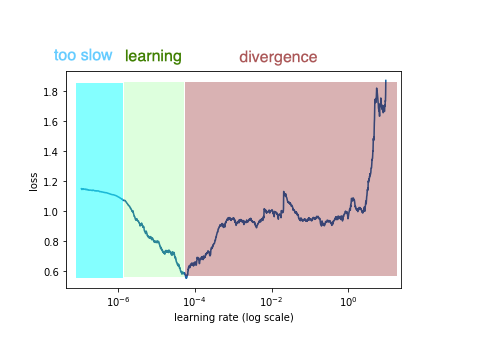
\includegraphics[width=0.8\textwidth]{diagrams/learning_rate2.png}
\caption{
Learning rate for \textit{distilbert} pre-trained model on airlines dataset.}
\label{fig:figlearningrate}
\end{figure}

\subsubsection{Training Strategy}
It is better to change the learning rate during training. In the beginning, when the model is bad, we want to find a better solution quickly. After some iteration, however, our model starts to be clever and it is unwanted to forget all and change the direction completely. Ktrain offers three possibilities of training - \textit{fit\_one\_cycle}, \textit{fit}, and \textit{autofit} (see Figure \ref{fig:strategies}).
\begin{figure}
\centering
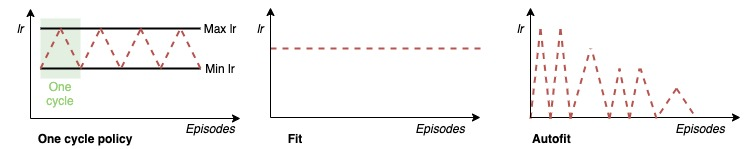
\includegraphics[width=1\textwidth]{diagrams/strategies.jpg}
\caption{
A comparison of different Ktrain training methods. On the left plot, learning rate is oscillating in every cycle between minimal and maximal learning rate. Cycle length can generally be different from epoch, but typically one cycle is one epoch long. The middle image shows just constant learning rate during whole training and the rightmost figure shows possibilities of autofit method to change learning rate after n periods without loss decrease (where n is a parameter).  
}
\label{fig:strategies}
\end{figure}
%TODO obrazek lepsi s porovnanim
 One cycle policy \cite{smith2018disciplined}goes from the lower bound to the upper bound in each cycle.
\textit{Autofit} method performs one cycle policy with cycle length equal to epoch for every epoch. It is also able to automatically decrease the learning rate if the loss on the validation set does not improve and stop training when it starts to diverge. The third method, \textit{fit}, is simple - it just uses the constant learning rate all the time.

\subsection{Experiments}
\label{sec:experiments}
In this section, different learning strategies effect is presented in a short overview. 
Experiments where performed for different learning rates and different strategies. 

Figure \ref{fig:acc_loss} plots progression of loss function and accuracy over 10 training epochs for tree different learning rates. For the \textit{fit} method, where constant learning rate is used, loss function starts to grow immediately after the first epoch, so further training just worsens results. One cycle policy for learning rates $4\cdot10^{-6}$ and $7\cdot10^{-6}$ is learning well for five or four epochs respectively, but best results are actually same or worse than one epoch with constant learning rate. Autofit starts to diverge, even when decrease of learning rate after 2 epochs with an increasing loss function was set for the greatest learning rate.

\begin{figure}[H]
\centering
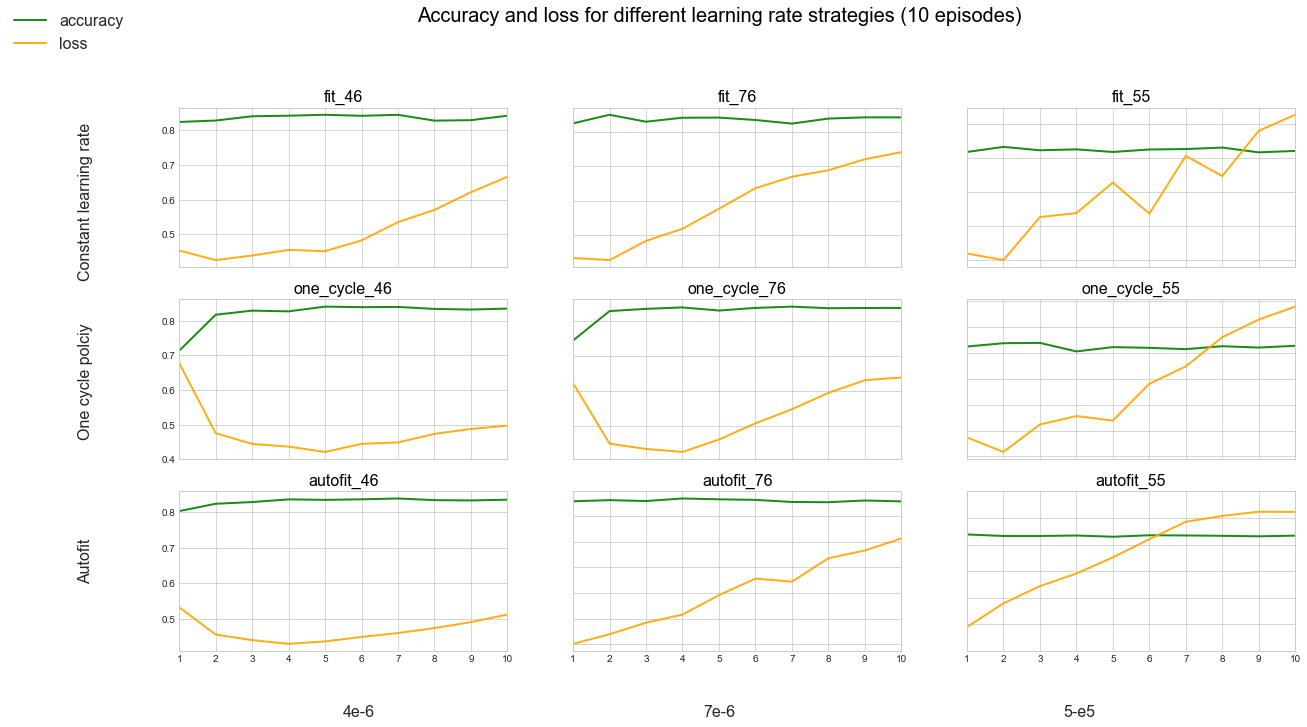
\includegraphics[width=1\textwidth]{diagrams/acc_loss.png}
\caption{ Loss and accuracy progress trough 10 training episodes.
}
\label{fig:acc_loss}
\end{figure}

There were performed other experiments using reduce of learning rate with different starting learning rate value. As starting on $8\cdot10^{-7}$ was slow, but with increasing learning rate over 20 episodes, starting with $6.25\cdot10^{-6}$ was to much and loss function grew for every episode. Neither of mentioned models was able to outperform the chosen one.


\par
For usage in Socneto, model \textit{fit\_76} from figure \ref{fig:acc_loss}, as it has the best accuracy. It is the model trained using only constant learning rate $7\cdot10^{-6}$ for 10 epoch. \\
\begin{center}
    

\begin{table}[H]
\label{table:resultsAnalysis}
\begin{tabular}{llll}
         & \textbf{precision} & \textbf{recall} & \textbf{f1 score} \\
\textbf{neutral}  & 0.87      & 0.82   & 0.84     \\
\textbf{positive} & 0.90      & 0.88   & 0.89     \\
\textbf{negative} & 0.94      & 0.87   & 0.96    
\end{tabular}
\caption{
Results for selected model for Socneto.}
\end{table}
\end{center}
As it is possible to see in table \ref{table:resultsAnalysis}, on the development data, the model is very good in recognizing negative texts (as the precision form negative is quite good) and the most hardly recognized are neutral posts.

\chapter{Extensibility Guide}\label{chapter:extensibility}

This document discusses an implementation of a custom data acquirer (Section~\ref{section:custom_da}) and a custom data analyser (Section \ref{section:custom_ds}). Each section introduces concrete contract that has to be followed (see Section~\ref{section:extensibility}). When each acquirer or analyser is registered, it can be used during a new job configuration (see Figure~\ref{job-fe})

\begin{figure}[H]\label{job-fe}
\centering
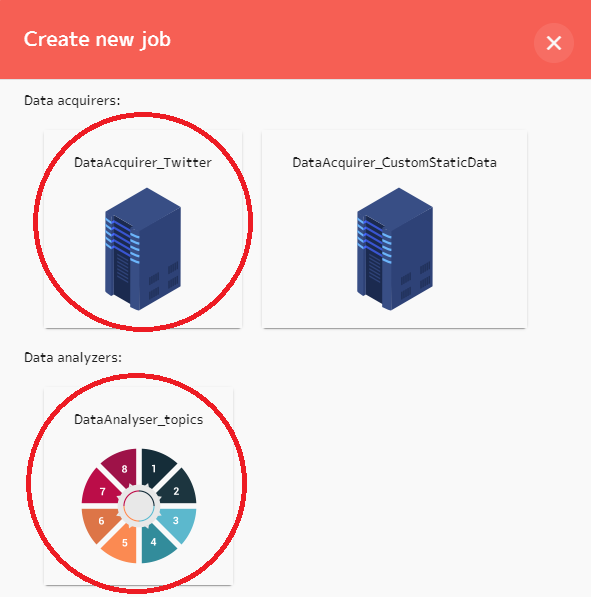
\includegraphics[width=0.7\textwidth]{diagrams/fe-job.png}
\caption{Screenshot of New Job form on Socneto front end. It shows all properly registered components}
\label{figure:monitoring-diagram}
\end{figure}

\section{Data Acquirer - QuoteLoader}\label{section:custom_da}

QuoteLoader loads data from a free API \url{http://quotes.rest/qod.json} returning random quotes.

\subsection{Contract}

\paragraph{Registration}

QuoteLoader sends registration request to the the topic\newline %\texttt{job\_management.registration.request}. \\ The registration request looks as follows:
\texttt{job\_management.registration.request}

\begin{lstlisting}[language=json,firstnumber=1]
{
  "componentId": "quoteLoaderDataAcquirer",
  "componentType": "DATA_ACQUIRER",
  "updateChannelName": "job_management.job_configuration.quoteLoaderDataAcquirer"
  }
}
\end{lstlisting}

Note that the \texttt{inputChannelName} is not present since QuoteLoader is data acquirer and does not have an input.

\paragraph{Starting the job}

QuoteLoader starts listening on a topic \newline
\texttt{job\_management.job\_configuration.quoteLoaderDataAcquirer}
 \\for a job like this:

\begin{lstlisting}[language=json,firstnumber=1]
{
    "jobId": "11d46859-3569-4bb1-9ec0-20eeac6ce132",
    "command": Start,
    "attributes":{},
    "outputChannelNames": [
        "job_management.component_data_input.storage_db",
        "job_management.component_data_input.some_analyser"]
}
\end{lstlisting}

Once the job notification arrives, QuoteLoader starts sending GET HTTP requests to \url{http://quotes.rest/qod.json}. QuoteLoader must remain listening to the topic while processing the newly arrived job. The endpoint returns JSON with the quote that looks like this (truncated for clarity):

\begin{lstlisting}[language=json,firstnumber=1]
{
    "quote": "You make a living by what you earn; you make a life by what you give.",
    "author": "Winston Churchill",
    "language": "en",
    "date": "2020-02-29",
    "id": "XZiOy4u9_g4Zmt7EdyxSIgeF"
}
\end{lstlisting}

The quote is then transformed into a post message and sent to both output channels \texttt{"job\_management.component\_data\_input.storage\_db"} and\newline \texttt{       "job\_management.component\_data\_input.some\_analyser"}.\\The post message looks like this:

\begin{lstlisting}[language=json,firstnumber=1]
{
  "id" : <new random uuid>,
  "jobId" : "11d46859-3569-4bb1-9ec0-20eeac6ce132", // from job notification
  "originalId" : "XZiOy4u9_g4Zmt7EdyxSIgeF", //quote id
  "text" : "You make a living by what you earn; you make a life by what you give.",
  "authorId" : "Winston Churchill",
  "language" : "en",
  "datetime" : "2020-02-29"
}
\end{lstlisting}
       
\paragraph{Stopping the job}

A stop job notification comes from the same topic as the start job notification. QuoteLoader listens on a topic \newline \texttt{job\_management.job\_configuration.quoteLoaderDataAcquirer} for a job like this:

\begin{lstlisting}[language=json,firstnumber=1]
{
    "jobId": "11d46859-3569-4bb1-9ec0-20eeac6ce132",
    "command": Stop
}
\end{lstlisting}

Quote loader stops the job while still listening on a the topic for new jobs.

\section{Data Analyser - Hashtags}\label{section:custom_ds}

This section describes on a real implementation, how can be a new analyser added to  Socneto.

\subsection{Contracts}

Hashtag analyser is implemented to simulate the easy extensibility of analysers. This component has a simple goal: compute frequencies of hashtags in posts.

\paragraph{Registration}

The analyser sends a registration request to the the topic \newline \texttt{job\_management.registration.request}. \\The registration request looks as follows:

\begin{lstlisting}[language=json,firstnumber=1]
{
  "componentId": "HashTags",
  "componentType": "DATA_ANALYSER",
  "inputChannelName": "job_management.component_data_input.HASH_TAG",
"updateChannelName": "job_management.job_configuration.HASH_TAG"
  }
}
\end{lstlisting}

\paragraph{Starting the Job}

The Hashtag analyser is stateless, so it does not need update messages. All posts are always analysed and sent to storage on a topic:\\ \texttt{job\_management.component\_data\_analyzed\_input.storage\_db}\\

\paragraph{Analysing posts}

When the post message is received, the module creates a frequency map of found hashtags and sends the analysis message to the storage
\\

\noindent
\textbf{Example post message:}


\begin{lstlisting}[language=json,firstnumber=1]
{
  "id" :"9e36b903-7f1b-43dd-b4f8-f64a8f95245d",
  "jobId" : "11d46859-3569-4bb1-9ec0-20eeac6ce132",
  "originalId" : "XZiOy888_g4Zmt7EdyxSazc",
  "text" : "#czech_castle #top09 Kalousek na hrad.",
  "authorId" : "Andrej",
  "language" : "cz",
  "datetime" : "2020-02-29"
}
\end{lstlisting}

\noindent
\textbf{Example analysis:}

\begin{lstlisting}[language=json,firstnumber=1]
{
  "postId": "9e36b903-7f1b-43dd-b4f8-f64a8f95245d",
  "jobId": "11d46859-3569-4bb1-9ec0-20eeac6ce132",
  "componentId": HashTags,
  "results": {
    "valueName": {
        "numberValue": null
        "textValue": null
        "numberListValue": null
        "textListValue": null
        "numberMapValue": {
                "czech_castle": 1,
                "top09": 1
        },
        "textMapValue": null
    }
  }
}
\end{lstlisting}
       
\paragraph{Stopping the Job}

Because this analyser is stateless, it does not need to work with the stop job procedure.

\subsection{Java Skeleton}\label{section:custom_ds}

The Hashtag analyser is implemented on  top of our prepared Java Spring skeleton for an easy analyser implementation. This implementation is stored in \textit{generic\_analyser} folder. There is a list of steps, that must be followed to integrate a new analyser into the platform from this skeleton.

\begin{itemize}
  
  \item A new analyser must have configured these properties \textit{in application.proper\-ties}:
  
  \begin{itemize}
  \item Unique component id
	\begin{itemize}
        \item property: \texttt{component.config.componentId}
    \end{itemize}
  
  \item Topic for new posts
    \begin{itemize}
	    \item property: \texttt{component.config.topicInput}
        \item conventionally with prefix: \texttt{job\_management.component\_data\_in\-put}
    \end{itemize}
  
  \item Topic for job updates
    \begin{itemize}
	    \item property: \texttt{component.config.topicUpdate}
        \item conventionally with prefix: \texttt{job\_management.job\_configuration}
   \end{itemize}
  
  \item Spring profile
    \begin{itemize}
	    \item property: \texttt{spring.profiles.active}
   \end{itemize}
  \item Output format (described in Section \ref{subsubsection:registration_analyser})
  
  \end{itemize}
  
  \item Orchestration is prepared and the only one thing is to implement the \texttt{cz.cuni.mff.socneto.storage.analyzer.Analyzer} interface. There are two methods, that must be overridden:
  \begin{itemize}
	    \item \texttt{Map$<$String, String$>$ getFormat()}
	    \begin{itemize}
	        \item an output format for registration message (the structure is described in Section \ref{subsubsection:registration_analyser})
        \end{itemize}
	    \item \texttt{$<$MapString, AnalysisResult$>$ analyze(String text)}
	    \begin{itemize}
	        \item input: a text to analyse
	        \item output: a result in the same format as the format returned in the method \textit{getFormat}
        \end{itemize}
   \end{itemize}
\end{itemize}

This approach should help an expert users of Socneto to implement a new analyser with reusing common and required parts of all analysers.

\chapter{Testing}\label{chapter:testing}

Socneto framework is tested on the following four levels, ordered from the lowest level to the highest:

\begin{itemize}
    \item Unit - Automatic tests of methods or classes
    \item Integration - Automatic tests of integration of multiple classes
    \item Component - Automatic tests of the whole component
    \item System - Manual tests of the whole application
\end{itemize}

\section{Requirements}

\begin{itemize}
    \item .Net Core 3.1 SDK
    \item .Net Core 2.2 SDK (for backend)
    \item Python 3.7.1
    \item Powershell Core 6.2.4
\end{itemize}


\section{Unit Tests}

\textbf{Job Management Service}
\\ \\
Test location: \texttt{<socneto-root-dir-path>/job-management/Tests}\\
Run tests command: 
\begin{lstlisting}[style=DOS]
dotnet test <socneto-root-dir-path>/job-management/Tests 
\end{lstlisting}
\vspace{\baselineskip}
\textbf{Backend}
\\ \\
Test location: \texttt{<socneto-root-dir-path>/backend/Tests}\\
Run tests command: \begin{lstlisting}[style=DOS]
dotnet test <socneto-root-dir-path>/backend/Tests
\end{lstlisting}
\vspace{\baselineskip}
\textbf{Data Acquirers}
\\ \\
All data acquirers shares the same code base therefore are all tested with the same unit tests.\\ \\
Test location: \texttt{<socneto-root-dir-path>/acquisition/DataAcquirer/Tests}\\
Run tests command: \begin{lstlisting}[style=DOS]
dotnet test <socneto-root-dir-path>/acquisition/DataAcquirer/Tests
\end{lstlisting}
\vspace{\baselineskip}
\textbf{Storage }\\
Test location: \texttt{<path-to-module>/src/test/java}\\
Run tests command: \begin{lstlisting}[style=DOS]
mvn test -DskipTests=false
\end{lstlisting}


\section{Integration Tests}


\textbf{Job Management Service}
\\ \\
Test location: \texttt{<socneto-root-dir-path>/job-management/Tests.Integration}\newline
Run tests command: \begin{lstlisting}[style=DOS]
dotnet test <socneto-root-dir-path>/job-management/Tests.Integration
\end{lstlisting}
\vspace{\baselineskip}
\textbf{Data Acquirers} \newline
\\
All data acquirers shares the same code base therefore are all tested with the same unit tests.\\ \\
Test location: \texttt{<socneto-root-dir-path>/acquisition/DataAcquirer/Tests.Inte\-gration}\newline 
Run tests command: 
\begin{lstlisting}[style=DOS]
dotnet test <socneto-root-dir-path>/acquisition/DataAcquirer/Tests.Integration
\end{lstlisting}

\section{Component Tests}

Component tests can be run separately, as described below, or at once with the following command: \\ \begin{lstlisting}[style=DOS]
<socneto-root-dir-path>/tests/component_tests/run_test_da.ps1
\end{lstlisting}
\vspace{\baselineskip}
\textbf{Job Management Service} \\ \\
Test location: \texttt{<socneto-root-dir-path>/tests/component\_tests/code/test\_da.ps1} \\
Run tests Powershell script:\\ \begin{lstlisting}[style=DOS]
<socneto-root-dir-path>/tests/component\_tests/run\_test\_da.ps1
\end{lstlisting}
\vspace{\baselineskip}
\textbf{Data Acquirers}
\\ \\
Test location: \texttt{<socneto-root-dir-path>/tests/component\_tests/code/test\_da.ps1}\\
Run tests Powershell script:\\ \begin{lstlisting}[style=DOS]
<socneto-root-dir-path>/tests/component\_tests/run\_test\_da.ps1
\end{lstlisting}
\vspace{\baselineskip}
\textbf{Data Analysers}
\\ \\
Test location: \texttt{<socneto-root-dir-path>/tests/component\_tests/code/test\_an.ps1}\\
Run tests Powershell script:\\ \begin{lstlisting}[style=DOS]
<socneto-root-dir-path>/tests/component\_tests/run\_test\_an.ps1
\end{lstlisting}
\vspace{\baselineskip}
\textbf{Backend}
\\ \\
Test location: \texttt{<socneto-root-dir-path>/tests/component\_tests/code/test\_be.ps1}\\
Run tests Powershell script:\\ \begin{lstlisting}[style=DOS]
<socneto-root-dir-path>/tests/component\_tests/run\_test\_be.ps1
\end{lstlisting}

\chapter{Discussion}

\section{Architecture}
% multiple services
Socneto was designed to be extensible, therefore a monolithic application was not a considered feasible. The domain of the application was split into dedicated services allowing them to run independently coordinated by one dedicated Job Management Service.

% why kafka
Socneto consists of multiple data acquirers streaming data to multiple data producers and eventually into the storage. It is unsuitable to use synchronous communication for streaming therefore Socneto internal communication is based upon asynchronous message broker Kafka. At the beginning, this decision was slowing us down, because it could solve more complex tasks than we needed. But in the end, we achieved our goal to have a scalable, distributed and extensible architecture. 

% db
The only change in the architecture during implementation was to remove the NoSQL database from the storage module, because it was not useful for any use-case and Elasticsearch is sufficient for the storing acquired data. If we had more time, there could be more research about choosing the right messaging broker, for example, we could use a more lightweight solution. Otherwise, this architecture satisfies a possible production usage. The only unimplemented part is authentication and authorization between FE, Backend, JSM and Storage modules.

\section{Infrastructure}
% 
Socneto was designed to run on premises. This gave us absolute freedom of the architectural and hosting aspects of the development. The university provided us with multiple Virtual Machines which were used to test and deploy Socneto. Given the fact that Socneto is a data processing framework, it could not be hosted on a single PC. 

The alternative to this decision was to run Socneto in some cloud platform. The disadvantages are:
\begin{itemize}
    \item The lack of professional experience with the application scope of the size of Socneto.
    \item The time required to get accustomed to cloud development.
    \item Unsuitability of the cloud for prototyping
    \item Limited options of free subscriptions and price of premium ones.
\end{itemize}
These disadvantages outweighted the advantages a cloud would have. The cloud is a infrastructure-as-a-service. All production grade features such as scaling, load balancing, security are supported out-of-the-box. The decision in favour of on premises deployment was based upon the fact that in this stage Socneto is not a production grade software making the use of the advantages limited.

% docker
Socneto design allows it to run in Docker - each component is hosted in a separated docker container. Docker (docker-compose) was chosen, because it provides fast deployment with easy configuration without requiring all installed dependencies. This approach can be extended with automatic testing and deployment pipeline, which is used in real-world projects. 
% We decided to not spend time implementing an automatic pipeline, because we didn't have a capacity for this. (this was moved to future work)

% technology freedom 
Important benefit is that each service can be implemented using different technology. In Socneto, each component is written in a language most suitable for the purpose of the given component. In this case, data analysers are based on python since it is the most popular language for data science related tasks. Java was used for data storing related service since it integrates best with Java based Elastic Search. Due to that there were no conflicts in the beginning of the project related to technological uniformity.


\section{Social Networks}
% why which social network
After the Cambridge Analytics issue \footnote{\url{https://en.wikipedia.org/wiki/Cambridge_Analytica}}, most social network providers limited their API usage which influenced the decision of which social networks to support. Socneto supports Twitter and Reddit. Twitter was chosen, because it offers easily accessible data with many customers for free and Reddit because it contains longer textual data with comments. Facebook was not used, because it restricted API was not possible to utilize for free.

Lately, social networks started to shift toward audiovisual content rather than textual. Supporting such network will introduce a whole new level of complexity and would impact every aspect of Socneto architecture. For that reason Socneto focuses only on textual data leaving space for future improvement. 

\section{Data Analysis}

As a part of this project, three text analyses where implemented - named entity recognition, sentiment analysis and latent Dirichlet analysis. We mainly used third-party libraries with existing pre-trained models. For sentiment analysis, fine-tuning of the model was performed together with the best model selection. We definitely do not have state-of-the-art solutions, but our analyses have a reasonable performance for usage and can be easily improved with more training (which include more time and also more training data).

\section{Market Potential}

% tohle patri spis do project timeline
%During implementation, we missed the fifth colleague, who was supposed to cover testing, deployment and real use cases. We managed to split his responsibilities among the member of the team which resulted in a reliable framework which proved itself to two subjects therefore it could be used by possible customers.

Development of Socneto has two directions. The first one is to open it to public and let each potential customer to build their personalized frameworks around it and monetize the support as many other projects already have done (most notable are Hadoop Ecosystem\footnote{\url{https://hadoopecosystemtable.github.io/}} and Project BlackLight\footnote{\url{http://projectblacklight.org/}})

The other is to extend it ourselves the way as our competitors did (as discussed in Section \ref{section:relatedWork}). Before we may sell Socneto to the first possible customer, we should extend analysers with more functionality (geographical data, image recognition) and also we have to cover other data sources (Instagram, Pinterest). The platform needs to improve security and all components need polishing. But the current state is prepared for further improvements.

\section{Summary}

Socento successfully delivered the specified functionality. Starting with acquisition of data from various sources and its following analysis with complex linguistic models performing sentiment analysis and topic modelling. The application fulfills requirements made to data storage and visualization. Extensibility was proved by implementing custom dataset acquirer and hasthag analyser on top of what was originally planned. 

To sum up the positive sides, the application is a well-designed data processing framework that  employs principles such as service oriented architecture, asynchronous messaging and NoSQL databases. Socneto uses modern platform for deployment making it easier for users' better integration. 

The weaker side of Socneto is the lack of security and proper user management expected from a production-grade software, but not essential for an academic project. Testing could be improved to give us a confidence that Socneto is ready for being used by customers.

\section{Future Work}

Socneto lack of production-grade features is currently the most pressing issue that should be solved before Socneto can be released. The problem with security and user management would be solved with migration to the cloud which would require some adjustments. It would also make it easier to implement continuous integration process.

In terms of the functionality, data acquirers could utilize more data offered by social networks such as geo codes, post statistics and comments. It could also start processing non textual data and implement analyses that would understand it. Socneto currently supports only primitive data flow with three steps. Some data acquirer gives data to some data analyser which then gives analyses to storage. This can be expanded to support custom data flow chaining compatible analysis. For example, the translation service is coupled with Twitter and Reddit data acquirers. It could be turned into a stand-alone component that would be part of the pipeline.  
\chapter{Conclusion}

This document presents an extensible platform for downloading and analysing data from social network. It established the field of interest, introduced competitors and the timeline of the project. It delivers comprehensive architectural and code documentation with an extensibility guide and discusses achieved results. In conclusion, Socneto was a successful project that served its developers as a ground for proving that university prepared them for their careers.
\newpage
\bibliographystyle{IEEEtran}
\bibliography{bibliography}
\newpage
\appendix
\chapter{Appendix}
%\setcounter{chapter}{1}
%\renewcommand\thesection{\Roman{section}}
%\renewcommand\thesubsection{\thesection.\Roman{subsection}}


\section{Entities}\label{appendix}

All entities are in JSON format, data types of values are inside $<$ and $>$ symbols.

\subsection{Registration Message}\label{subsection:registrationrequest}

\begin{lstlisting}[language=json,firstnumber=1]
{
  "componentId": <string>,
  "componentType": <DATA_ACQUIRER or DATA_ANALYSER>,
  "updateChannelName": <string>,
  "inputChannelName": <string>,
  "attributes": <json object>
  }
}
\end{lstlisting}

\subsection{Job Configuration}

\begin{lstlisting}[language=json,firstnumber=1]
{
    "selectedDataAcquirers":[<string>],
    "selectedDataAnalysers":[<string>],
    "topicQuery": <string>,
    "jobName": <string>,
    "attributes":{
        "acquirer_1":{
            "parameter1": <string>
        }
        ...
    }
}
\end{lstlisting}

\subsection{Update Message}\label{subsection:notification}

\begin{lstlisting}[language=json,firstnumber=1]
{
    "jobId": <uuid>,
    "command": <'Start' or 'Stop'>,
    "attributes":{
        "attribute_1": <string>,
        ...
    },
    "outputChannelNames": [<string>]
}
\end{lstlisting}

\subsection{Post Message}\label{subsection:postmessage}

\begin{lstlisting}[language=json,firstnumber=1]
{
  "id" : <uuid>,
  "jobId" : <uuid>,
  "originalId" : <long>,
  "text" : <string>,
  "originalText" : <string>,
  "authorId" : <string>,
  "language" : <string>,
  "datetime" : <datetime>
}
\end{lstlisting}

\subsection{Analysis Message}\label{section:analysisMessage}

\begin{lstlisting}[language=json,firstnumber=1]
{
  "postId": <uuid>,
  "jobId": <uuid>,
  "componentId": <string>,
  "results": {
    "valueName": {
        "numberValue": <double>,
        "textValue": <string>,
        "numberListValue": [<double>],
        "textListValue": [<string>],
        "numberMapValue": {<string,number>},
        "textMapValue": {<string,string>}
    }
  }
}
\end{lstlisting}

\subsection{Log Message}\label{section:logMessage}

eventType values: FATAL, ERROR, WARN, INFO, METRIC

\begin{lstlisting}[language=json,firstnumber=1]
{
  "componentId": <string>,
  "eventType": <string>,
  "eventName": <string>,
  "message": <string>,
  "timestamp": <datetime>,
  "attributes": {<any object>}
}
\end{lstlisting}
\newpage
\section{Detailed specification as approved}
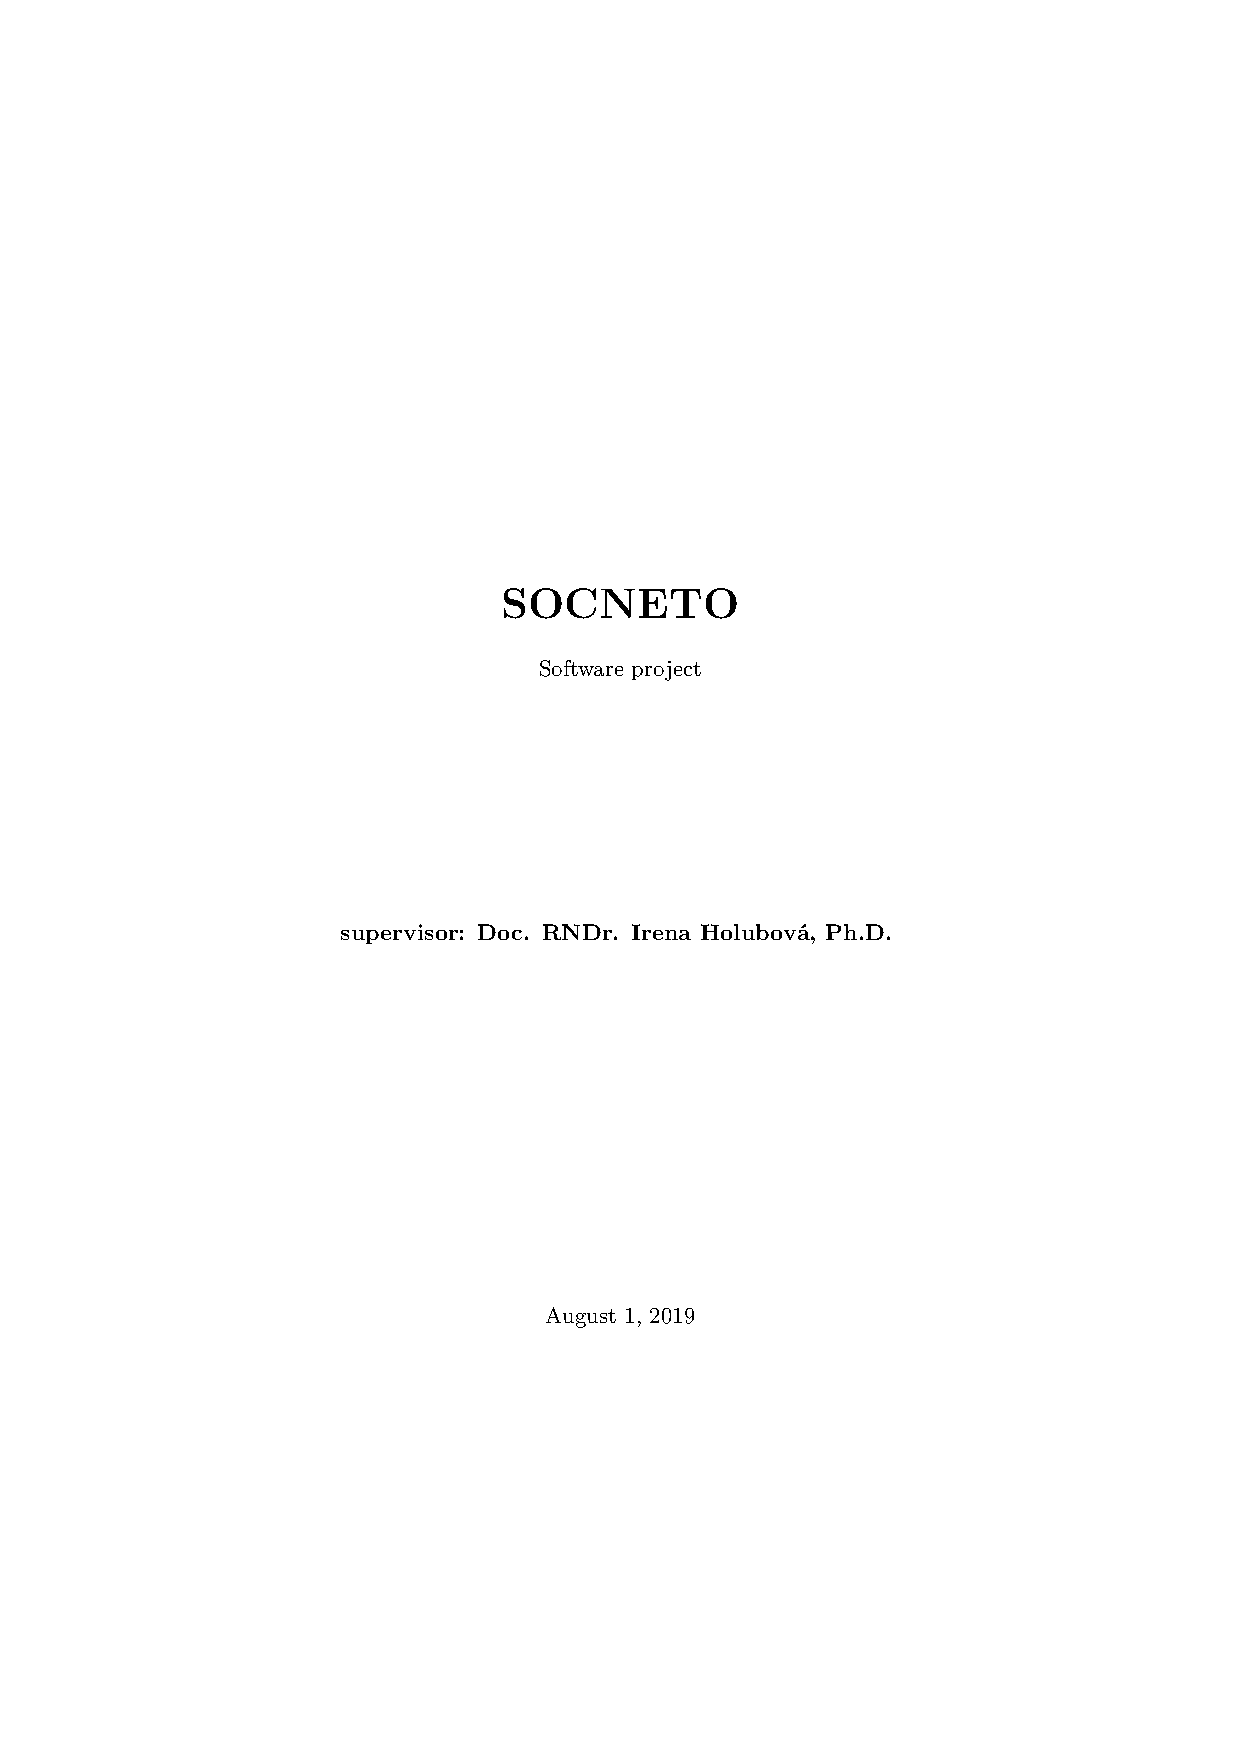
\includepdf[pages=-]{specification.pdf}


%\addcontentsline{toc}{section}{References}

\newpage
%\listoftodos

\end{document}

